%*********************第二章******************
\chapter{使用``目标候选''提高跟踪器的尺度和宽高比适应力}
\label{chapbmvc}

\section{引言}
绪论已经介绍过,视觉跟踪器是视频监控、人机交互、智能导航等应用领域至关重要的基础。
从上世纪80年代的KLT跟踪器\upcite{lkoptflow, klt2},到最新提出的深度学习跟踪器\upcite{deepimage, deeptrack},
视觉跟踪已经被研究了几十年。
但随着应用需求的不断提升,应用场景的日趋复杂,很多问题仍然未得到有效解决。
跟踪器对目标物体的尺度和宽高比的适应力就是这些问题之一。

跟踪算法的基础研究一般面向最为通用的跟踪器类别,即``短时间、单目标、无模型''跟踪器。
``短时间''是一个相对概念,通常意指用于跟踪的是较短的视频序列(通常从几百帧到几千帧),而不是直接进行长时间的在线跟踪。
``单目标''即被跟踪的目标物体只有一个,跟踪过程中不考虑其它物体的位置和状态。
``无模型''指的是不依赖跟踪目标的任何先验信息,不在跟踪前对目标物体进行任何建模。
跟踪算法中最为通用的结果表示方式是``边界框'',即在图像帧中紧密包围目标物体的矩形框。
跟踪过程中,目标物体可能发生复杂的运动、旋转、形变等。
体现在结果上,就是边界框的位置、尺度和宽高比发生变化。
如果跟踪器边界框的尺度和宽高比无法随物体发生变化,那么跟踪结果仅能体现出物体的位置信息,而无法描述其它物体状态。
除此之外,不准确的边界框还将导致跟踪过程中不准确的目标/背景分割。
过多的非目标物体信息可能包含在边界框中,而部分目标物体信息却可能在边界框外。
这些误差将在物体描述中积累,积累到一定程度,跟踪器将出现偏移(Drifting),整个跟踪过程很可能就此失败。
图\ref{scalearerror}就展示了一个尺度和宽高比误差的可视化例子。
因此,跟踪器对目标尺度和宽高比的适应力对跟踪精度有着决定性的作用。

\begin{figure}[htb]
\centering
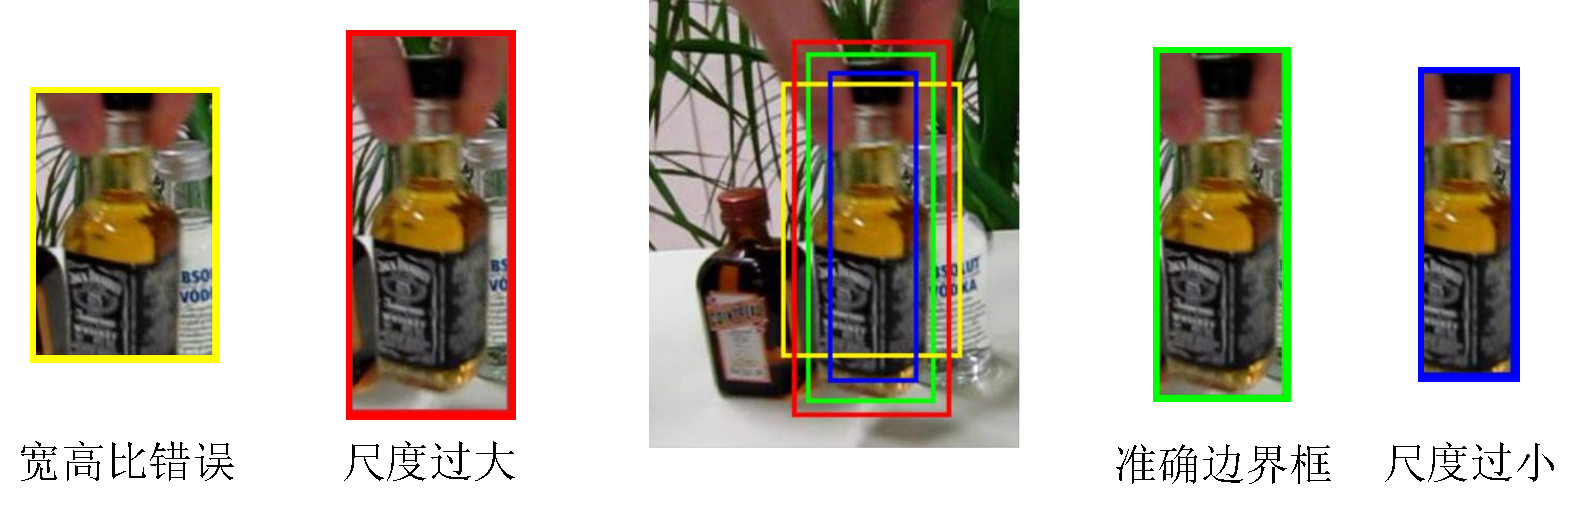
\includegraphics[width=12.5cm]{scaleaspect.pdf}
\caption{尺度和宽高比误差的可视化例子}
\label{scalearerror}
\end{figure}

为了应对视觉跟踪应用中的诸多挑战,跟踪算法正变得越来越复杂。
然而近年提出的基于相关滤波的跟踪器\upcite{mosse,csk,kcf,dsst,act,samf,pbcf} 在取得上佳性能的同时,却十分简单和快速。
这些跟踪器的核心部分都是一个具有分辨能力的滤波器,其输出的卷积结果能够显示出输入图像和跟踪目标的相似度。
由于频率域的点对点操作等价于时间域(图像处理中为空间域)的卷积操作,
上述滤波器能够极其高效地辨识所有循环位移后的输入图像。
但是,滤波器的输入必须是固定大小的图像块,因此基于相关滤波的跟踪器天生缺乏对于目标尺度和宽高比变化的适应力。
尽管一些能够适应尺度变化的变型\upcite{dsst,samf,pbcf}已经出现,但是它们仍局限于预定的尺度采样方式,不够灵活。
此外,在本章已知的范围内,除了\cite{pbcf}以外还没有相关滤波跟踪器能够解决对于目标宽高比的适应性问题。

在物体检测领域,近来具有顶级性能的物体检测系统\upcite{rcnn,spp}均采用了``目标候选''方法来提取可能包含目标物体的候选区域。
该类方法可以在没有任何先验知识的情况下,在输入图像中提取任意尺度、宽高比的候选边界框,如图\ref{detectionproposalres}所示。
目标候选方法不仅能够避免对大量的边界框进行分类,还能预先滤除大部分错误的边界框,大幅提高检测精度\upcite{dpsurvey,dpcompare}。
在本章中,目标候选生成器EdgeBoxes\upcite{edgeboxes}将被融入跟踪器中,
以提升跟踪器对尺度和宽高比的适应力。

\begin{figure}[htb]
\centering
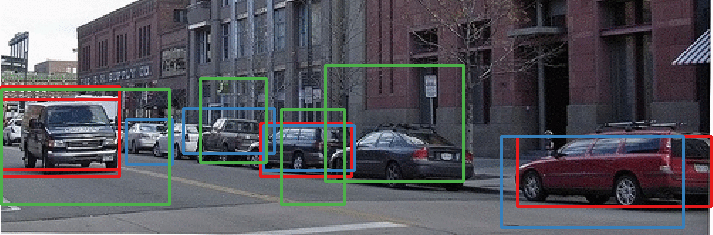
\includegraphics[width=13cm]{detectionproposalres.png}
\caption{生成``目标候选''的可视化例子}
\label{detectionproposalres}
\end{figure}

本章选用EdgeBoxes的原因在于,在众多目标候选生成器中,它不仅具有顶级的生成精度,
而且还具有足以应用于跟踪任务的生成速度(考虑到跟踪任务中的待检测范围远小于物体检测任务)。
此外,由于EdgeBoxes将物体边界作为生成目标候选的唯一线索,它在跟踪任务中还具有以下优势。
首先,它不需要任何预先学习过程,因而适用于通用的视觉跟踪器。
其次,作为物体线索的边界,同时也是推测被跟踪目标物体的位置和大小的线索。
最后,它包含了大量可调节的参数,使得可以针对跟踪任务进行调优。

本章中,KCF\upcite{kcf}这一典型的基于相关滤波的跟踪器将作为跟踪器的主体框架。
通过对输入滤波器的图像特征进行增强,以及采用更为鲁棒的跟踪器模型更新方法,
KCF的辨别力将变得更加鲁棒和准确,足以对灵活的目标候选进行分类。
初步确定目标所在位置后,EdgeBoxes将被用于在其附近生成目标候选。
这些候选边界框经过一个过滤步骤后,将被输入KCF进行再次辨别,以提取出最优的目标候选。
最后,通过一个阻尼更新过程,最优候选边界框将被用于确定最终的目标位置、尺度和宽高比。
本章最终将得到一个集成了目标候选生成器的全新跟踪器,它在公开的大规模测试集中取得了顶级的精度,
并且达到了20.8 FPS(每秒处理的帧数)的跟踪速度。

本章的内容安排如下:第2节介绍与本章紧密相关的现有研究工作;
第3节介绍本章跟踪器框架的基础\pozhehao 核化相关滤波器KCF;
第4节对KCF进行优化,以适应对目标候选的分类任务;
第5节介绍如何将目标候选生成器EdgeBoxes高效地融入跟踪框架中;
第6节将对本章方法进行实验评测和分析;
最后在第7节进行本章的总结。

\section{相关研究}
\subsection{跟踪器的尺度和宽高比适应力}
根据绪论中对跟踪器各模块的功能分析可以看出,运动模型是决定一个跟踪器的尺度和宽高比适应力的关键。
\cite{survey51}基于光流跟踪算法,已被广泛应用于图像对准(Image Registration)。
它通过增量式对齐(Incremental Alignment)来计算两帧中目标物体图像块的仿射变换(Affine Transformation)。
由于仿射变换的参数包含6个自由度,因此该跟踪器可以感知目标物体的位移、尺度变化和旋转。
LSK跟踪器\upcite{lsk}在每一帧中都会预先``猜测''一个目标中心位置并采样候选图像块,
然后使用Mean-Shift聚类方法优化该猜测,以最大化候选图像块和匹配模板的相似度。
由于Mean-Shift优化过程会根据多种尺度反复进行,因此LSK跟踪器能够成功判断当前目标的尺度大小。
上述两个跟踪器中,物体的运动都是通过计算或者优化过程直接得到的,因此其运动模型属于隐式模型。

ASLA\upcite{asla}和SCM\upcite{scm}均采用仿射变换来描述两帧间的目标运动。
与\cite{survey51}根据光流跟踪结果直接计算仿射变换不同,这两个跟踪器将仿射变换的6个参数用6个独立的高斯分布进行建模。
然后,跟踪器将通过不断采样仿射变换参数并进行验证的方式,寻找最为合适的目标位置和尺度。
这种按照概率分布来采样目标状态参数,然后以目标当前状态更新概率分布的方式,属于典型的点滤波(Particle Filtering)运动模型。
VTD\upcite{vtd}跟踪器会同时考虑目标的位置和尺度变化,并用两个高斯分布来分别建模平滑和突发的目标运动。
这两个点滤波运动模型将配合多个不同的观察模型,得出多个跟踪结果,
并通过马尔科夫链蒙特卡洛(Markov Chain Monte Carlo)方法整合出一个最终结果。

此外,还有部分跟踪器使用了特殊方法来获得尺度和宽高比适应力。
为了应对物体非刚性形变带来的大幅度尺度和宽高比变化,HBT\upcite{houghtrack}将图像分割方法加入了跟踪过程。
根据霍夫森林(Hough Forest)得出的反向映射向量将投票决定目标物体的中心位置,
而中心位置将作为前景点输入图割算法Grabcut,以对目标物体和背景进行分割。
由于图像分割得到的是目标物体的细致轮廓,因此HBT可以准确适应目标的尺度和宽高比变化。
但是图像分割计算开销巨大,使得HBT难以用于实时跟踪场景。
TLD\upcite{tld, tldjournal}跟踪算法将Fern随机森林检测器和光流跟踪器进行了整合。
Fern随机森林检测器通过滑动窗口的方式搜索整幅帧图像,找出可能包含目标物体的边界框;
光流跟踪器则根据多个目标特征点的运动,估计目标的整体运动。
这两个模块均能适应目标的尺度和宽高比变化。

\subsection{基于相关滤波的跟踪器}
基于相关滤波的跟踪器通常选择密集采样作为运动模型,即是说,它们通过在图像中密集地采样候选区域并进行辨别,
来检测目标物体的当前位置和状态。
因此,密集采样的模式(例如采样时边界框的大小、形状是否可变)决定了跟踪器对尺度和宽高比的适应力。
MOSSE跟踪器\upcite{mosse}将经过随机仿射变换的目标物体图像作为训练集,用于初始化它的相关滤波器。
但是在跟踪过程中,采样边界框的尺度和宽高比不再变化,滤波器仅用于检测目标的当前位置。
KCF\upcite{kcf}跟踪器是CSK\upcite{csk}的一个扩展版本,它通过利用图像块中的循环模式进行卷积操作,取得了极高的跟踪效率。
KCF还利用``核技巧(Kernel Trick)''来增强了传统的相关滤波器,同时使得滤波器支持多通道的特征。
但是,它仍然没有解决尺度的适应力问题。
作为CSK的另一个固定尺度扩展版本,ACT\upcite{act}采用颜色名(Color Naming)作为特征,并使用了特征压缩方法提高跟踪效率。
此外,ACT还提出了一个更加鲁棒的模型更新策略以提高精度。

SAMF\upcite{samf}在KCF的基础上,通过在采样时加入几种预定义的尺度变化来解决KCF的尺度适应力问题。
相关滤波器将对这些不同尺度的采样样本进行辨别,以找出最佳的目标位置和尺度大小。
不同于SAMF,DSST\upcite{dsst}将两个独立的相关滤波器结合在了一起:一个基于MOSSE,仅用于估计目标位置;
另一个为一维相关滤波器,仅用于确定目标物体尺度。
在每一帧中,DSST首先利用第一个滤波器确定目标位置。
然后在该位置处采样不同尺度的图像块组成``尺度金字塔'',并将其输入第二个滤波器中以估计尺度。
对比SAMF和DSST,可以看出DSST的尺度检测会更加地准确和快速。
因为相关滤波器具有辨别力,可以显式地区分出各个尺度的置信度,并且可以在频率域更快地进行计算。
但是,这两个基于相关滤波的跟踪器都没有针对目标的宽高比变化进行处理。
\cite{pbcf}中提出的跟踪器通过使用多个独立的相关滤波器来同时跟踪目标物体的多个部分,
并将各个滤波器的输出整合为一个响应图。
随后,跟踪器在响应图中按照高斯分布采样不同的位置、尺度和宽高比,并使用一个贝叶斯框架对采样样本进行评价,
以确定目标物体的当前状态。
显然,上述跟踪器均依赖于预先定义好的采样模式,因而灵活性严重受限,无法处理突发、快速的尺度和宽高比变化。

STC\upcite{stc}是一个例外,它在估计目标尺度时使用的运动模型为隐式模型。
严格来讲,STC并不是基于相关滤波的,但是其推导出的核心算法与相关滤波器十分类似。
它对目标和目标周围区域的上下文时空关系进行了重新建模,并将尺度的变化显式地体现在了模型中。
因此尺度变化可以被直接计算出来而无需通过采样,但是宽高比的变化仍然无法被感知。

\section{使用核化相关滤波器进行视觉跟踪}
\label{kcfsec}
作为本章跟踪器的主体框架和基础,核化相关滤波器KCF的主要目标是训练一个线性模型:
\begin{equation}
f(\mathbf{z})=\left\langle\mathbf{w}, \mathbf{z}\right\rangle ,
\label{kcfeq1}
\end{equation}
其中函数值$f(\mathbf{z})$显示了输入图像块$\mathbf{z}$与目标物体的相似程度,即线性模型的响应值。
$\left\langle\cdot, \cdot\right\rangle$代表内积,
$\mathbf{w}$为该线性模型的参数矩阵。
公式\ref{kcfeq1}即是KCF的观察模型,即判断候选图像块是否包含目标物体的模块。
KCF将上一帧的目标物体边界框进行放大,得到一个上下文窗口,然后根据该窗口提取图像块。
该图像块的每一次循环位移都将产生一个候选图像块$\mathbf{z}$,并将被输入观察模型,以计算其中包含目标的概率。
显然,若当前帧中目标物体在上下文窗口内,那么目标物体一定位于某一个循环位移后的图像块的中心,
该图像块的$f(\mathbf{z})$也应当具有最大值。
可视化的例子如图\ref{kcf1}所示。显然,循环位移就是KCF的运动模型。
由于会对所有循环位移进行辨别,因此它还是一种密集采样运动模型。

\begin{figure}[htb]
\centering
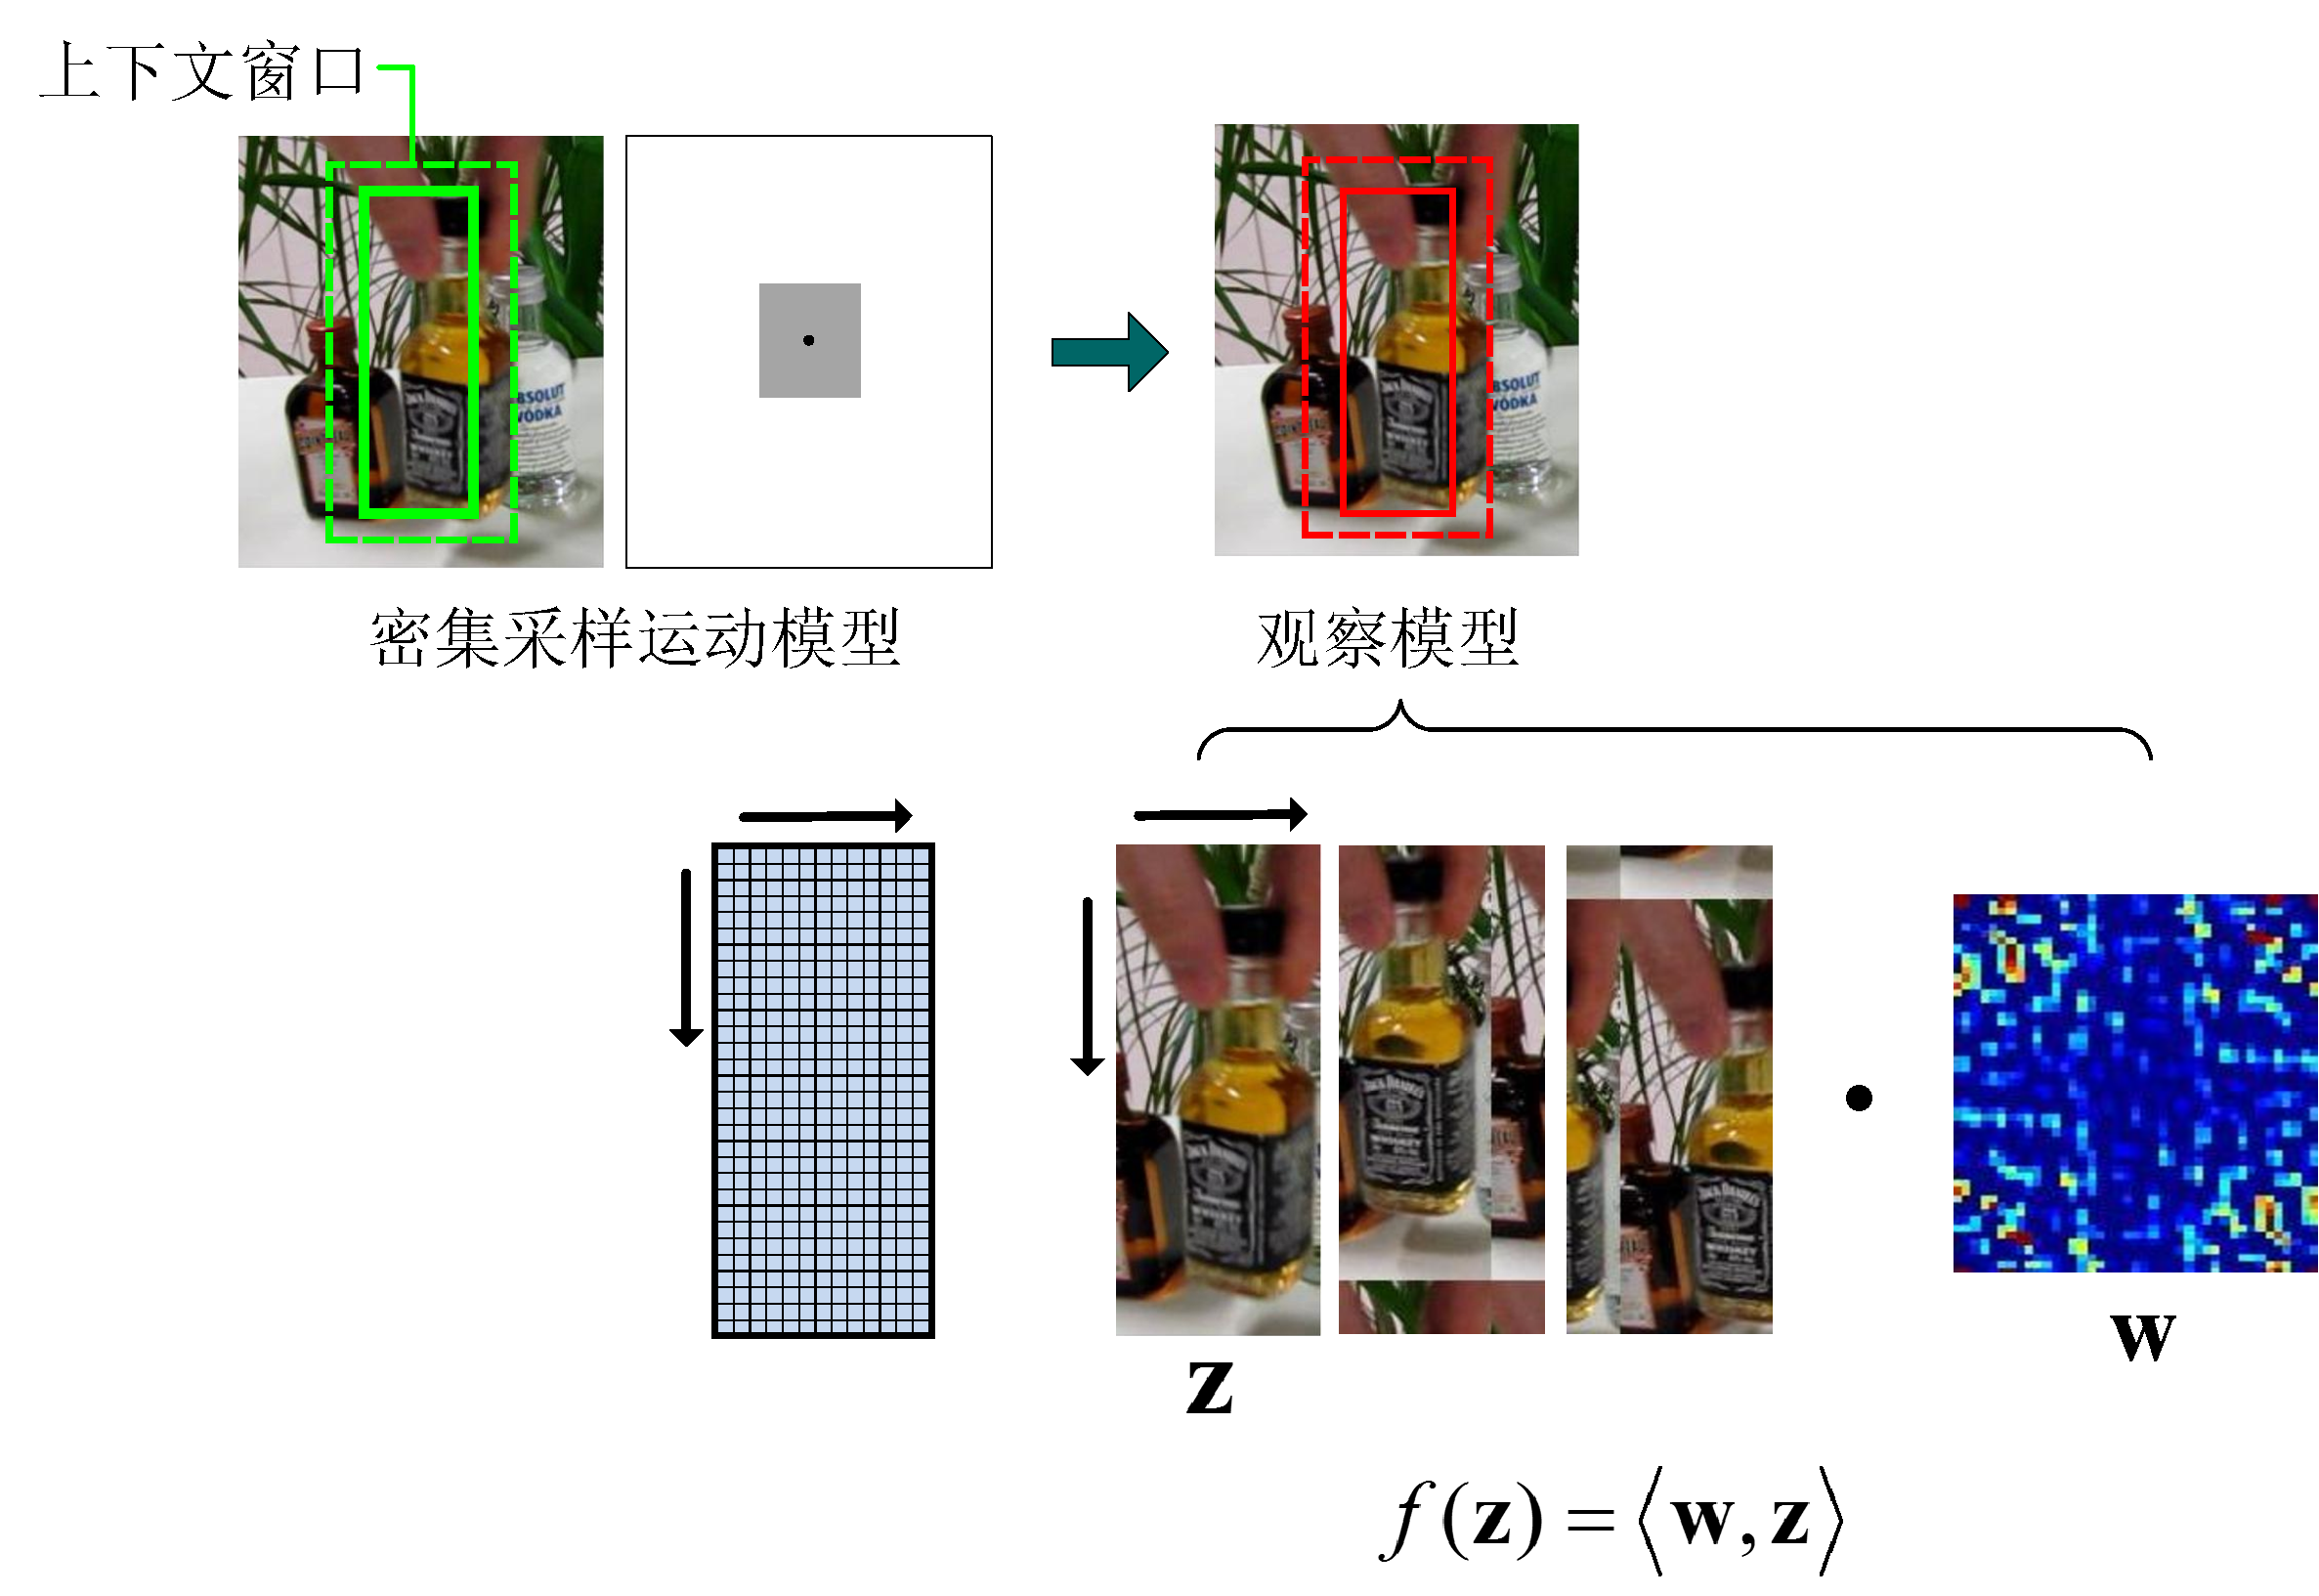
\includegraphics[width=11cm]{kcf1.pdf}
\caption{KCF的运动模型和观察模型}
\label{kcf1}
\end{figure}

求解参数矩阵$\mathbf{w}$的过程,就是求解``岭回归(Ridge Regression)''问题的过程。该求解或者说训练的目标函数为:
\begin{equation}
	\underset{\mathbf{w}}{\min}\,\sum_{m,n}\left(f(\mathbf{x}_{m,n})-y_{m,n}\right)^{2}+\lambda\left\Vert \mathbf{w}\right\Vert ^{2}.
	\label{rrmin}
\end{equation}
$\mathbf{x}_{m,n}$是用于训练的图像块,$\lambda$被称作规则化参数(Regularization Parameter),用于防止过拟合。
$y_{m,n}$是回归目标,即对于输入的$\mathbf{x}_{m,n}$所期望的$f(\mathbf{x}_{m,n})$值。
在KCF中,$\mathbf{x}$代表目标物体图像块,即一个``真值''。
$\mathbf{x}_{m,n}$是由$\mathbf{x}$纵向循环位移$m-1$个像素,再横向循环位移$n-1$个像素所得到的图像块。
显然$\mathbf{x}_{1,1}=\mathbf{x}$,因此其对应的$y_{1,1}$应当具有最大值,即$y_{1,1}=1$。
若将所有的$y_{m,n}$组成一个矩阵$\mathbf{y}$,那么理想情况下,$\mathbf{y}$应当符合一个将峰值循环位移到左上角的二维高斯函数。

KCF通过使用高斯核函数,将公式\ref{kcfeq1}变换到了对偶空间(Dual Space):
\begin{equation}
\begin{aligned}
	f(\mathbf{z})=\left\langle\mathbf{w}, \mathbf{z}\right\rangle&=\sum_{m,n}\alpha_{m,n}\left\langle\mathbf{z},\mathbf{x}_{m,n}\right\rangle=\sum_{m,n}\alpha_{m,n}\ g\negthinspace\left(\mathbf{z},\mathbf{x}_{m,n}\right),\label{kcf-kernelmodel}
\end{aligned}
\end{equation}
其中$g\negthinspace\left(\cdot, \cdot\right)$代表高斯核函数,它取代了原式中的内积计算。
相对应的,KCF的运动模型和观察模型也变为图\ref{kcf2}所示。
计算$f(\mathbf{z})$值的过程,实际上变为了将候选图像块$\mathbf{z}$(图中标记为\textbf{C})和每一个训练图像块$\mathbf{x}_{m,n}$进行对比的过程,
参数矩阵$\mathbf{w}$也被新参数$\alpha_{m,n}$所组成的矩阵$\boldsymbol{\alpha}$所替代。
而训练图像块集合中,循环位移较小的必然与原目标物体图像块相似,成为了正样本(图中标记为\textbf{P});循环位移较大的则成为了负样本(图中标记为\textbf{N})。

\begin{figure}[htb]
\centering
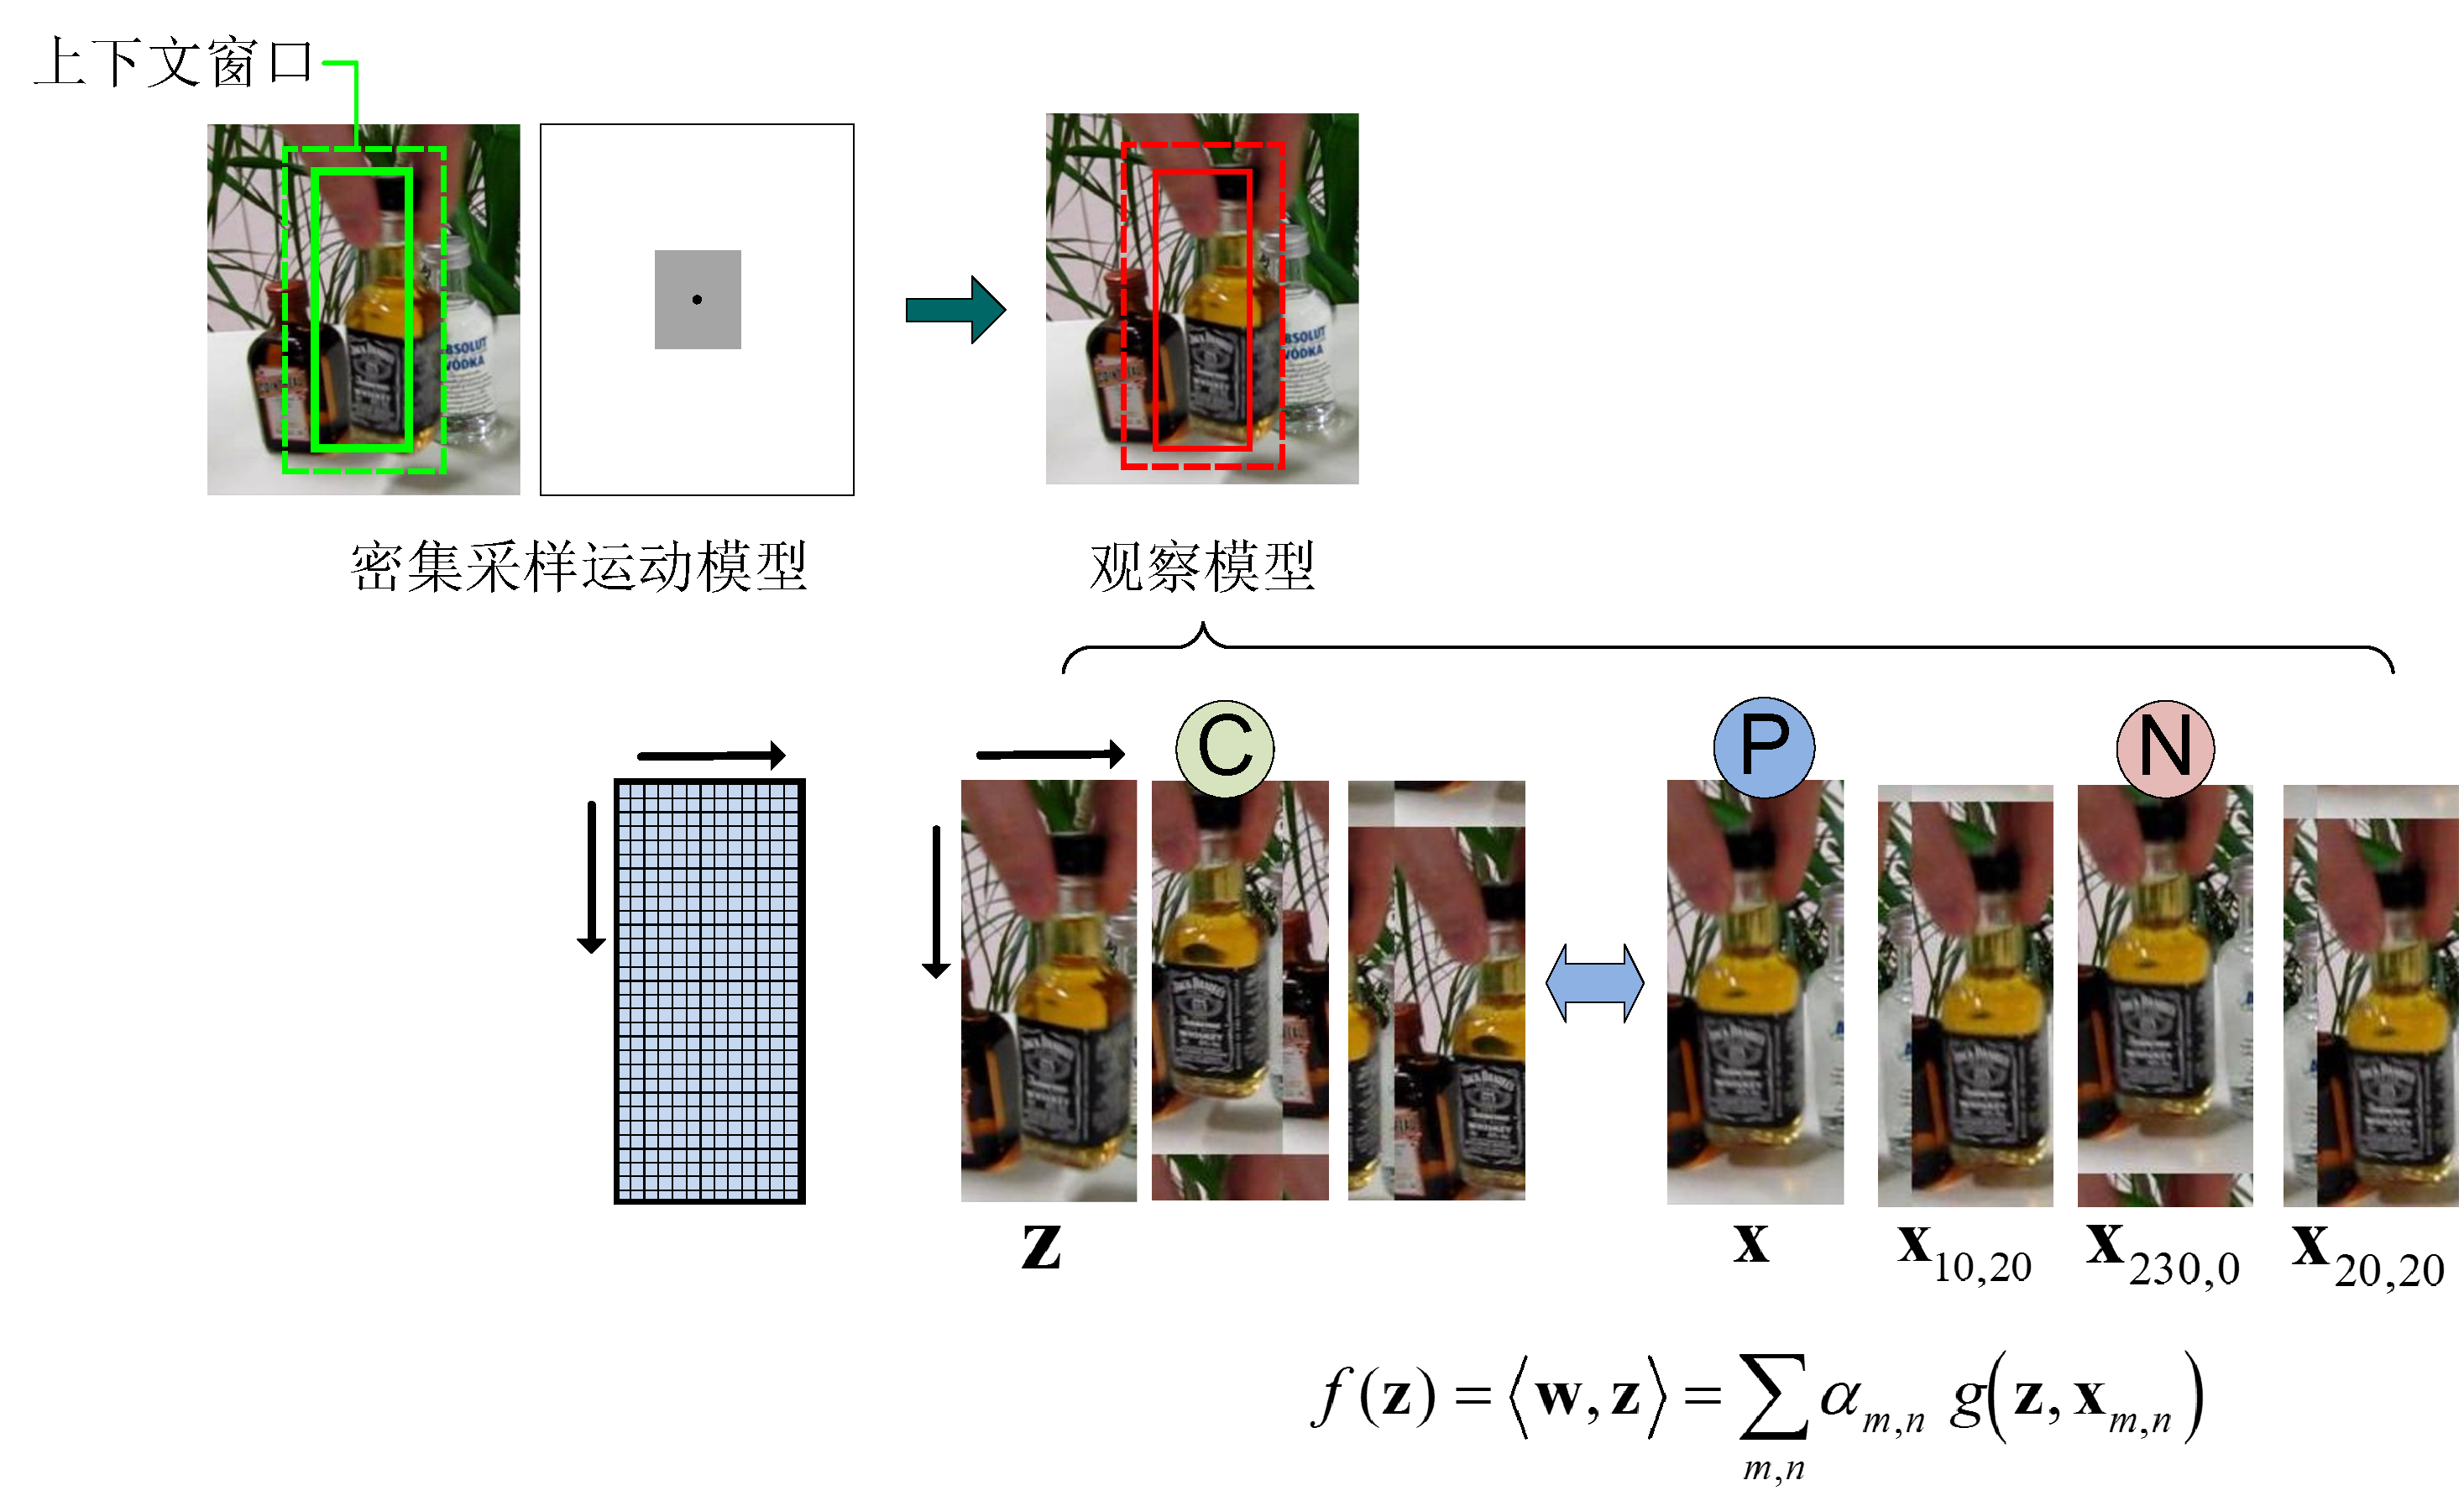
\includegraphics[width=13cm]{kcf2.pdf}
\caption{使用高斯核后的KCF运动模型和观察模型}
\label{kcf2}
\end{figure}

通过利用各个$\mathbf{x}_{m,n}$间的循环关系,以及卷积定理(Convolution Theorem),公式\ref{rrmin}的解为:
\begin{equation}
	\hat{\boldsymbol{\alpha}}=\frac{\hat{\mathbf{y}}}{\hat{\mathbf{k}}{}^{\mathbf{x}_{1,1}\mathbf{x}_{1,1}}+\lambda}.\label{kcf_learning}
\end{equation}
上式中的$\hat{\cdot}$代表离散傅里叶变换(DFT),$\mathbf{k}$ 代表核化相关算子,其定义为:
\begin{equation}
\begin{aligned}
%	\mathbf{k}^{\mathbf{x' x''}}=\exp\left(-\frac{1}{\sigma^{2}}\left(\left\Vert \mathbf{x'}\right\Vert ^{2}+\left\Vert \mathbf{x''}\right\Vert ^{2}-2\mathcal{F}^{-1}\left(\sum_{c}\,\hat{\mathbf{x'}}_{c}^{*}\cdot\hat{\mathbf{x''}}{}_{c}\right)\right)\right), \label{kcf-kr}
	&\mathbf{k}^{\mathbf{x' x''}}=
	&\exp\left(-\frac{1}{\sigma^{2}}\left(\left\Vert \mathbf{x'}\right\Vert ^{2}+\left\Vert \mathbf{x''}\right\Vert ^{2}
	-2\mathcal{F}^{-1}\left(\sum_{c}\,\hat{\mathbf{x'}}_{c}^{*}\cdot\hat{\mathbf{x''}}{}_{c}\right)\right)\right), \label{kcf-kr}
\end{aligned}
\end{equation}
式中$\sigma$是高斯核函数的带宽,$\mathcal{F}^{-1}$代表离散傅里叶逆变换,${*}$代表复共轭算子,
下标$c$代表图像特征向量的第$c$个通道, $\exp$即指数函数。
公式\ref{kcf-kr}中的所有运算操作,包括$\exp$,都是逐元素进行的。
公式\ref{kcf_learning}将负责训练相关滤波器,即在第一帧中用用户标注出的或者检测到的目标物体图像块初始化相关滤波器。

同样利用循环关系和卷积定理,KCF可以同时计算出输入图像块$\mathbf{z}$的所有循环位移所对应的响应值。
也就是说,公式\ref{kcf-kernelmodel}可变换为:
\begin{equation}
	\hat{\mathbf{f}}(\mathbf{z})=\hat{\mathbf{k}}^{\overline{\mathbf{x}}\mathbf{z}}\cdot\hat{\boldsymbol{\alpha}},\label{kcf-detection}
\end{equation}
其中$\overline{\mathbf{x}}$被称作当前目标外观。
由于目标物体外观在跟踪中会不断变化,因此公式\ref{kcf-kernelmodel}中的$\mathbf{x}$也会不断更新,并记为$\overline{\mathbf{x}}$。
$\mathbf{z}$的所有循环位移的响应值$f$组成了矩阵$\mathbf{f}$,
且各个响应值在$\mathbf{f}$中的位置,与循环位移的像素数目相对应,即$\mathbf{f}[m,n]=f(\mathbf{z}_{m,n})$。
因此,根据$\mathbf{f}$中最大元素所在的位置,可以找出最接近当前目标外观的$\mathbf{z}_{m,n}$,
从而直接推断出目标物体中心在上下文窗口中的位置。
公式\ref{kcf-detection}是KCF的核心,将负责在每一帧中检测目标物体的中心位置。
而它又是由参数矩阵$\boldsymbol{\alpha}$和当前目标外观$\overline{\mathbf{x}}$所共同决定的,
因此这两个矩阵也被称作``KCF的模型''。

每当在新的一帧中跟踪到目标物体后,KCF都会更新自己的模型,以适应光照变化、目标旋转、形变等导致的目标外观变化。
KCF的模型更新策略非常简单直接,就是进行线性插值。
记当前帧中目标物体图像块为$\mathbf{x}_i$,对于参数矩阵,首先重新训练一个参数矩阵$\boldsymbol{\alpha}_i$,然后进行线性插值:
\begin{equation}
	\hat{\boldsymbol{\alpha}_i}=\frac{\hat{\mathbf{y}}}{\hat{\mathbf{k}}{}^{\mathbf{x}_i\mathbf{x}_i}+\lambda}, \\ \ \ \ 
	\boldsymbol{\alpha}=\eta{\boldsymbol{\alpha}_i} + ( 1-\eta )\boldsymbol{\alpha}.
	\label{kcf_learning2}
\end{equation}
对于目标外观,则直接进行线性插值:
\begin{equation}
\overline{\mathbf{x}}=\eta\mathbf{x}_i+(1-\eta)\overline{\mathbf{x}}.
\label{kcf_appearlearning}
\end{equation}


\section{图像特征整合和鲁棒更新}
在跟踪过程中加入目标候选生成器后,相关滤波器需要辨别的不仅是循环位移后的图像块,
还包括各种尺度大小和宽高比的目标候选。
由于候选图像块的灵活性和数量增加,各种干扰因素也将增加,对相关滤波器的精度和鲁棒性也提出了更高的要求。

为了提升精度,本节将首先加强KCF的目标描述。
KCF所使用的``梯度直方图(HOG)''特征被扩展为HOG、亮度和颜色名三者结合的混合特征。
这种特征整合的方法在SAMF\upcite{samf}和ACT\upcite{act}中均有使用,但是本节不对特征进行压缩。
这三种特征的简要介绍如下:
\begin{compactitem}
\item{\textbf{亮度}:要计算亮度,需要先将彩色图像转换为灰度图像。假设图像块按RGB三个通道存储,则一个像素的灰度可计算为:
$0.2989 * R + 0.5870 * G + 0.1140 * B$。随后,将每个像素的灰度值减去整个图像块的平均灰度值,即得到了各个像素的亮度值。}
\item{\textbf{梯度直方图}\upcite{hog}:在亮度图的基础上,首先对于每一个像素点,计算其横向和纵向的亮度梯度。
然后根据横、纵亮度梯度,计算出每个像素的梯度方向。之后将图像分为$4\times4$细胞单元(Cell)组成的网格,
并在每一个细胞单元中对9个离散的梯度方向进行投票。每个像素点的投票均具有权值,且该权值就是梯度的大小。
最后将多个细胞单元组合成较大的区块,并对这些区块中的梯度方向投票进行统计,得出梯度直方图特征。}
\item{\textbf{颜色名}\upcite{colornaming}:之所以将这种特征命名为颜色名,是因为它将所有的颜色按照语言学分为了11类,
即11类人类常用的颜色名字。这样的颜色分类更接近于人类的感知,且已经在物体检测\upcite{colornaminguse2}和动作识别\upcite{colornaminguse1}领域取得了很好的效果。这里直接利用\cite{colornaming}中的方法将RGB 3个通道的值向11个颜色名通道进行映射,
得到颜色名特征。}
\end{compactitem}
将这三种特征同时用于目标描述的原因是它们之间有很好的互补性:
亮度,顾名思义,描述的是各个像素的明亮程度,但是缺乏对不同颜色的区分度;
梯度直方图更着重于描述图像中的轮廓和形状,但是难以区分亮度和颜色;
颜色名是当前物体分类常用的颜色特征,有着明显优于传统RGB颜色表达的性能。

整合上述三种图像特征的方法比较直接,即对于一个图像块提取出三种特征后,将特征的各通道拼接存储。
例如原彩色图像块的每一个像素有R、G、B三个通道,故图像块存储为高$\times$宽$\times$3的三维数组。
提取特征并且整合后,由于三种特征共计有42个通道,图像块变为高$\times$宽$\times$42的三维数组。
在训练参数矩阵(公式\ref{kcf_learning})和评价候选图像块时(公式\ref{kcf-detection}),
只需要按照公式\ref{kcf-kr}的最后一项,对特征的各个通道进行分别处理即可。

如\ref{kcfsec}节所述,KCF采用简单的线性插值作为模型更新策略。
这种更新方法已经被证明是不够理想的\upcite{act},
因为每次模型更新时(公式\ref{kcf_learning2}),仅考虑了当前帧中的目标物体外表图像,
而之前帧中的目标外表的贡献,将按照学习速率$\eta$的指数级函数不断减小。
显然,这种更新策略是不够鲁棒的。
当跟踪出现偏移,或者目标外表突发剧烈变化时,KCF原来积累的准确模型将被迅速污染,从而很可能导致更大的跟踪偏移。

为了提高KCF的相关滤波器的鲁棒性,本节将把线性插值方法替换为ACT中的鲁棒更新方法。
在更新模型的参数矩阵$\boldsymbol{\alpha}$时,假设当前帧为第$i$帧,则从第$1$帧到当前帧的所有目标物体图像块可记为$\{\mathbf{x}_j : j=1, ..., i\}$。
%所有参数矩阵可记为$\{\boldsymbol{\alpha}_j : j=1, ..., i\}$。
更新参数矩阵的过程变为最小化以下目标函数的过程:
\begin{equation}
\begin{aligned}
	&\underset{\boldsymbol{\alpha}}{\min}\,\sum_{j=1}^{i}\phi_j(\Vert\mathbf{f}(\mathbf{x}_j)-\mathbf{y}\Vert^{2}+\lambda \left\langle\boldsymbol{\alpha}, \boldsymbol{\alpha}\right\rangle)=
	\\
	&\underset{\boldsymbol{\alpha}}{\min}\,\sum_{j=1}^{i}\phi_j(\Vert\mathcal{F}^{-1}(\hat{\mathbf{k}}^{\mathbf{x}_i\mathbf{x}_j}\cdot\hat{\boldsymbol{\alpha}})-\mathbf{y}\Vert^{2}+\lambda \left\langle\boldsymbol{\alpha}, \boldsymbol{\alpha}\right\rangle).
	\label{act-cost}
\end{aligned}
\end{equation}
该目标函数同时考虑了当前帧和所有历史帧中的目标物体图像块,
其实质为参数矩阵$\boldsymbol{\alpha}$对于所有帧中目标物体外表的平方误差加权和。
$\phi_j$即是权值,这里将其直接设置为学习速率$\eta$。

为了能够最小化上述目标函数,经过推导(详见\cite{act}),新的参数矩阵更新公式为:
\begin{equation}
\begin{aligned}
	&\hat{\boldsymbol{\alpha}_N}=\eta\hat{\mathbf{k}}^{\mathbf{x}_i \mathbf{x}_i} \cdot \hat{\mathbf{y}} + (1-\eta){\hat{\boldsymbol{\alpha}_N}};
	\\
	&\hat{\boldsymbol{\alpha}_D}=\eta\hat{\mathbf{k}}^{\mathbf{x}_i \mathbf{x}_i} \cdot (\hat{\mathbf{k}}^{\mathbf{x}_i \mathbf{x}_i} +
	\lambda) + (1-\eta){\hat{\boldsymbol{\alpha}_D}}.\label{kcfdp-updating}
\end{aligned}
\end{equation}
其中$\hat{\boldsymbol{\alpha}_N}$和$\hat{\boldsymbol{\alpha}_D}$分别为频率域$\boldsymbol{\alpha}$的分子和分母,即$\hat{\boldsymbol{\alpha}}={\hat{{\boldsymbol{\alpha}_N}}}/{\hat{{\boldsymbol{\alpha}_D}}}$。
值得注意的是,虽然所有历史帧中的目标图像块都在公式\ref{act-cost}中显式地考虑了,
但它们隐含在了迭代更新过程(公式\ref{kcfdp-updating})中,因此每次更新$\boldsymbol{\alpha}$时仅需要当前帧中的目标物体图像。
而KCF模型的另一部分,目标外观$\overline{\mathbf{x}}$,仍然按照公式\ref{kcf_appearlearning}进行线性插值式的更新。

\section{将``目标候选''嵌入跟踪器中}
\label{wholeprocesssec}
原KCF跟踪器在经过特征整合和鲁棒更新的优化后,将足以胜任对目标候选的辨别。
因此本节将把目标候选生成器EdgeBoxes嵌入优化后的KCF跟踪框架中,以同时利用目标候选的灵活性和优化后的KCF的准确辨别力。
嵌入目标候选生成器后的整个跟踪过程可视化地展示在了图\ref{process}中。

\begin{figure}[htb]
\centering
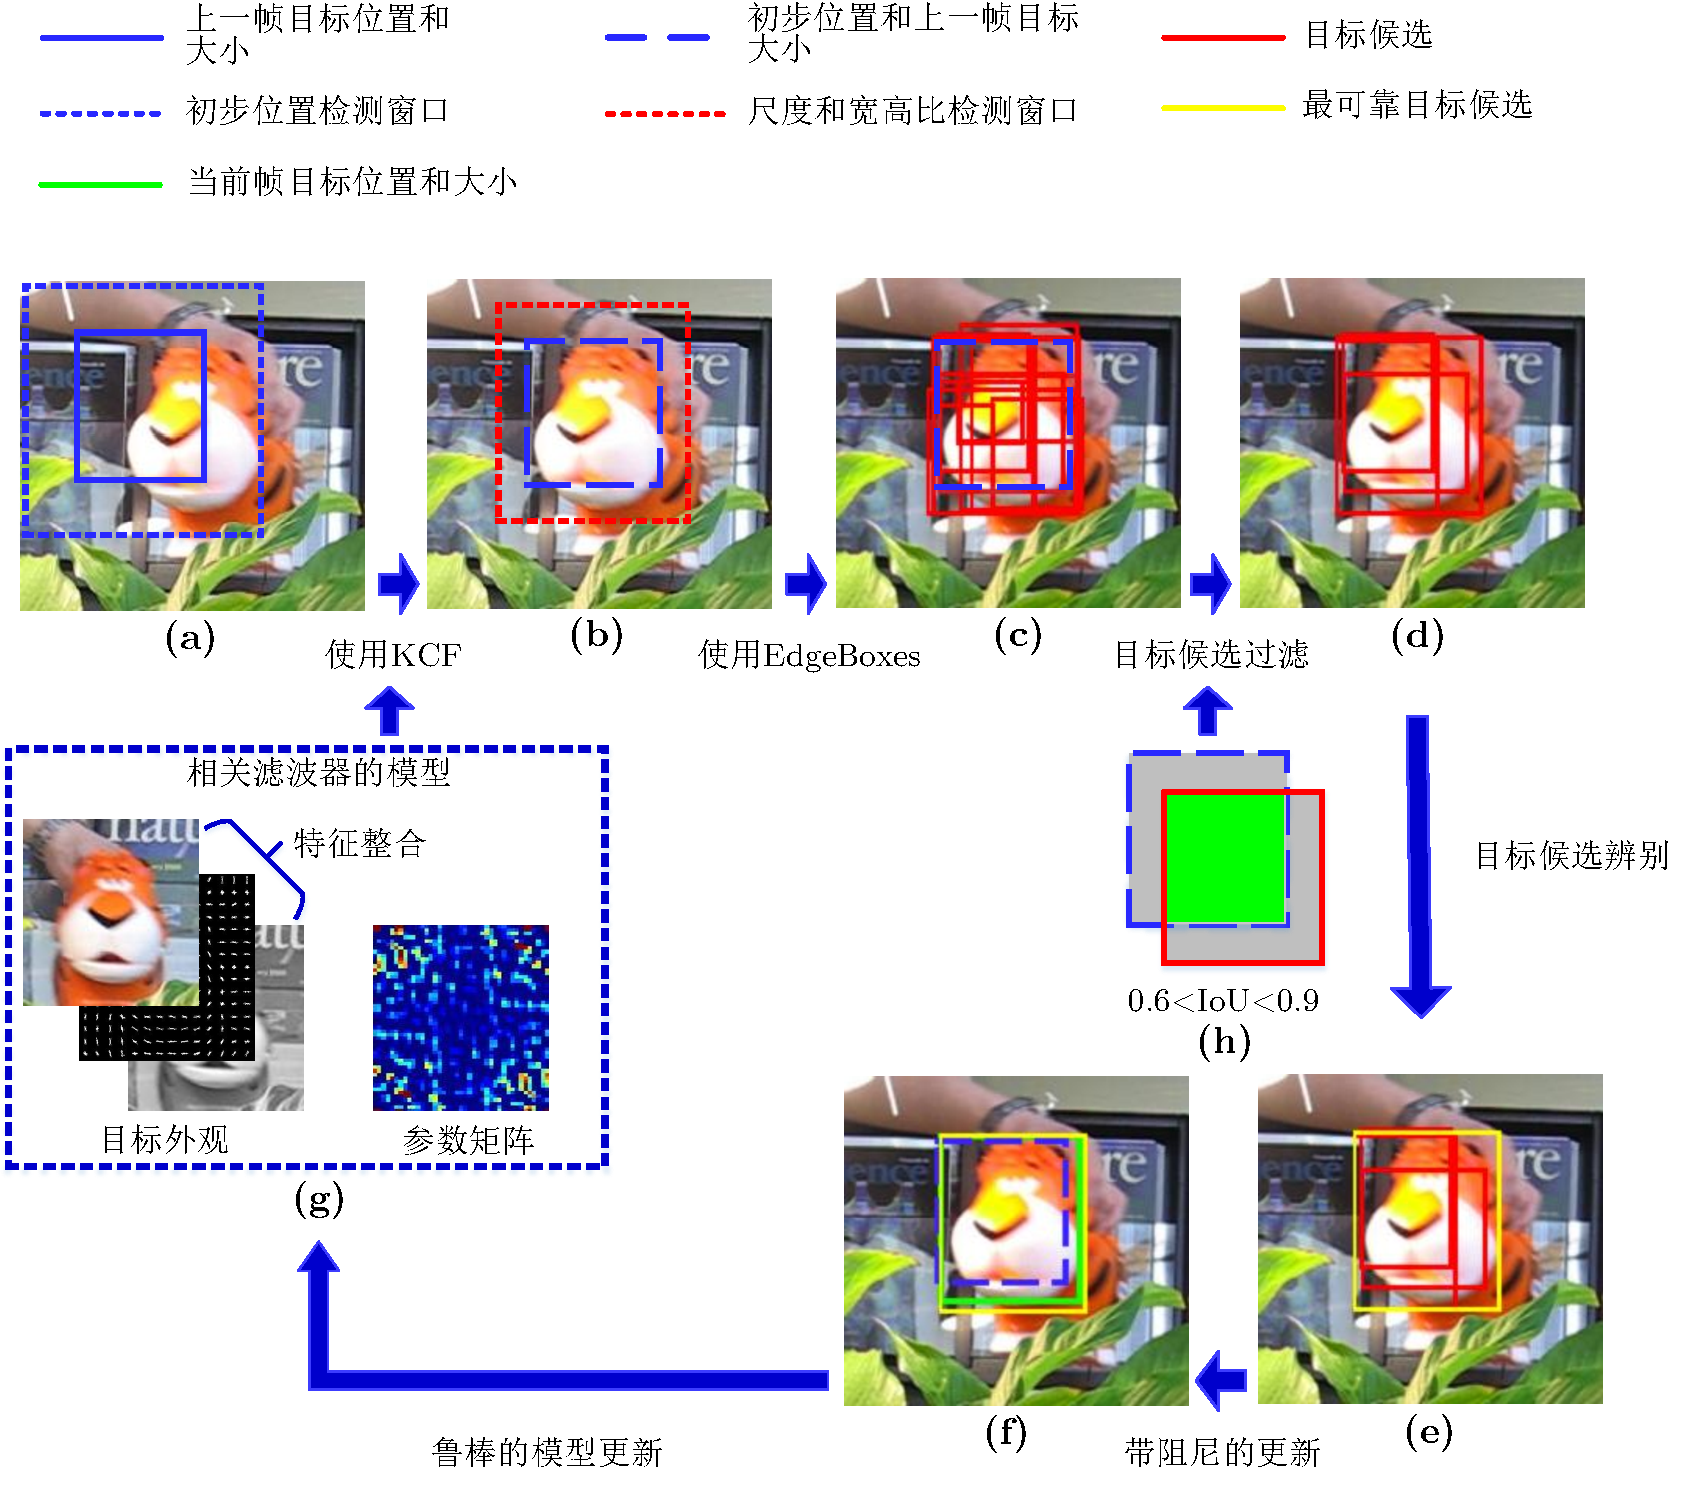
\includegraphics[width=15cm]{process-full.pdf}
\caption{本章跟踪器的可视化跟踪过程}
\label{process}
\end{figure}

在初始化时,第一帧中,记用户标注的或者目标检测得到的目标物体边界框大小为$w_1\times h_1$ ,
中心位于$\mathbf{l}_1$。
将该边界框扩大为$s^dw_1\times s^dh_1$,即得到了位于$\mathbf{l}_1$的上下文窗口。
这里的$s^d$被称为尺度因子,必须大于$1$以包含一定上下文信息,且覆盖下一帧中目标物体可能出现的位置。
为了初始化KCF的模型,此时将根据该上下文窗口提取出图像块$\mathbf{x}_1$,并用$\mathbf{x}_1$初始化参数矩阵${\boldsymbol{\alpha}}$ (公式\ref{kcf_learning})。
至于目标外观$\overline{\mathbf{x}}$,将其直接初始化为$\mathbf{x}_1$。

跟踪过程开始后,每当新的一帧(记为第$i$帧)到来时,
首先根据上一帧中的目标位置$\mathbf{l}_{i-1}$和目标大小$w_{i-1}\times h_{i-1}$,
设置一个中心位于$\mathbf{l}_{i-1}$,大小为$s^dw_{i-1}\times s^dh_{i-1}$的``初步位置检测窗口'',如图\ref{process}(a)所示。
然后根据该窗口提取图像块$\mathbf{z}^d$。
由于跟踪过程中,检测到的目标物体大小会不断变化,因此需要利用双线性插值(Bilinear Interpolation)
将 $\mathbf{z}^d$缩放到$s^dw_1\times s^dh_1$,才能利用无尺度适应力的KCF相关滤波器。
将KCF应用于图像块$\mathbf{z}^d$之后(公式\ref{kcf-detection}),
即可根据$\mathbf{f}$中最大元素的位置,判断出新的目标位置$\mathbf{l}^d_i$。
该目标位置称作``初步位置'',其对应的$\mathbf{f}$中最大元素值记为$v$。

下一步如图\ref{process}(b)所示,以初步位置$\mathbf{l}^d_i$为中心,$s^ew_{i-1}\times s^eh_{i-1}$为大小,构建一个``尺度和宽高比检测窗口''。
$s^e$也是一个尺度因子,但是应当设置得比$s^d$小,因为目标物体尺度的变化通常小于其位移。
根据尺度和宽高比检测窗口提取图像块$\mathbf{z}^p$后,将其输入目标候选生成器EdgeBoxes中。
如图\ref{process}(c)所示,EdgeBoxes将会输出大量的目标候选,即大量可能包含物体的边界框。
这些边界框已按照各自所得``分数''进行了排序,而该分数代表的就是边界框内包含物体的置信度。

对于EdgeBoxes输出的边界框,本节仅提取其前$N$个,并且对它们进行过滤:
计算每一个目标候选边界框与``初步目标物体边界框''的重叠率,如果重叠率大于0.9或者小于0.6,则将该目标候选剔除。
这里的初步目标物体边界框位于$\mathbf{l}^d_i$,大小为$w_{i-1}\times h_{i-1}$,
即一个位于初步位置,大小等于前一帧中目标大小的边界框。
如图\ref{process}(h)所示,重叠率使用IoU(Intersection over Union)进行度量,
其计算方式为将两个边界框的交集面积除以它们的并集面积。
IoU大于0.9的边界框几乎和初步目标物体边界框相同,无需纳入考虑;
而IoU小于0.6的边界框很有可能是错误的目标候选,或者其中包含的是非目标物体,均需要被剔除。

如图\ref{process}(d)所示,通过过滤后的目标候选数目已大幅下降。
但是,仍然需要用相关滤波器对这些目标候选进行再次辨别,才能找出图\ref{process}(e)中所示的``最可靠目标候选''。
对于每一个经过过滤的目标候选边界框,按尺度因子$s^d$进行扩大,并从当前帧中提取出对应的图像块,记为$\mathbf{p}$。
由于$\mathbf{p}$可能具有任意的尺度和宽高比,因此也需要将它缩放到$s^dw_1\times s^dh_1$后,才能使用相关滤波器进行辨别。
辨别一个目标候选图像块和当前目标外观的相似度时,使用下式:
\begin{equation}
	f(\mathbf{p})=\text{sum}(\mathbf{k}^{\overline{\mathbf{x}}\mathbf{p}}\cdot{\boldsymbol{\alpha}}),\label{kcfdp-eval}
\end{equation}
这里的$\text{sum}(\cdot)$代表对矩阵中所有元素的叠加操作,
$f()$和公式\ref{kcf-kernelmodel}中的$f()$意义相同,是一个代表着$\mathbf{p}$和$\overline{\mathbf{x}}$的相似度的标量。
由于这里仅需要对目标候选图像块本身进行辨别,而无需辨别它的所有循环位移,因此用公式\ref{kcfdp-eval}来代替公式\ref{kcf-detection}。
事实上,公式\ref{kcfdp-eval}就是公式\ref{kcf-detection}转换到空间域的结果。
在辨别完所有目标候选之后,本节将找出具有最大$f$值(记为$f_{max}$)的目标候选,
并记录其中心位置为$\mathbf{l}^{p}_i$,大小为$w^p_i\times h^p_i$。

如果$f_{max}$小于$v$,说明最可靠的目标候选边界框的准确性仍然不如``初步目标物体边界框''。
此时应放弃所有目标候选,认为初步位置$\mathbf{l}^d_i$就是当前帧中的目标位置$\mathbf{l}_i$,
且当前目标物体大小$w_i\times h_i$不变,仍然等于$w_{i-1}\times h_{i-1}$。
如果$f_{max}$大于$v$,则通过一个带阻尼的更新过程,将初步目标物体边界框和最可靠目标候选相结合:
\begin{equation}
\begin{aligned}
	%\mathbf{l}_i=\gamma\mathbf{l}^p_i+(1-\gamma)\mathbf{l}^d_i;\ \ \ 
	&\mathbf{l}_i=\mathbf{l}^d_i+\gamma(\mathbf{l}^p_i-\mathbf{l}^d_i);\\ 
	%(w_i, h_i)=\gamma(w^p_i, h^p_i)+(1-\gamma)(w_{i-1},h_{i-1}).
	&(w_i, h_i)=(w_{i-1},h_{i-1})+\gamma((w^p_i, h^p_i)-(w_{i-1},h_{i-1})). \label{kcfdp-damping}
\end{aligned}
\end{equation}
上式的$\gamma$为阻尼因子,其作用如图\ref{process}(f)所示。
用带阻尼的更新来最终确定目标的位置和大小,可以防止过于敏感的目标状态变化,同时还能降低跟踪错误或是目标候选错误带来的影响,
从而让跟踪器更为鲁棒。

在当前帧中完成跟踪后,还需要提取一个新的目标物体图像块来更新KCF的参数矩阵$\boldsymbol{\alpha}$和目标外观$\overline{\mathbf{x}}$。
显然,该图像块位于新目标位置$\mathbf{l}_i$,大小为$s^dw_i\times s^dh_i$,可被记为$\mathbf{x}_i$。
将$\mathbf{x}_i$输入公式\ref{kcfdp-updating},即可鲁棒地更新KCF的参数矩阵$\boldsymbol{\alpha}$;
而更新目标外观$\overline{\mathbf{x}}$则需要根据公式\ref{kcf_appearlearning}。
完成模型更新后,将进入针对下一帧的循环。

除了图\ref{process}所示的可视化过程,本节的跟踪过程还规范化地列在了算法\ref{algorithm}中。
更多可视化的目标候选辨别和带阻尼更新的例子可见图\ref{rejection}。
图\ref{rejection}还清楚地展示出了目标候选方法是如何让本章的跟踪器适应尺度和宽高比变化的。
正是由于目标候选的极大灵活性,本章的跟踪器可以轻易地找出被遮挡的目标(图\ref{rejection}右上),
并且还能准确地框出旋转的目标(图\ref{rejection}左下)。

\begin{algorithm}[htb]
	\begin{flushleft}
		{{}\textbf{输入:}}{\small \par}
		{\quad{}}{{\ } $F_i$: 图像帧}{\small \par}
		{\quad{}}{{\ } $(\mathbf{l}_{i-1}, w_{i-1}, h_{i-1})$: 在上一帧中紧密包围目标物体的边界框}{\small \par}
		%	 in format ``(center location, width, height)''.}{\small \par}
		{\quad{}}{{\ } $\boldsymbol{\alpha}$, $\overline{\mathbf{x}}$: 之前的模型(参数矩阵和目标外观)}{\small \par}
		\vspace{0.1in}
		{{}\textbf{输出:}}{\small \par}
		{\quad{}}{{\ } $(\mathbf{l}_{i}, w_{i}, h_{i})$: 在当前帧中紧密包围目标物体的边界框}{\small \par}
		{\quad{}}{{\ } $\boldsymbol{\alpha}$, $\overline{\mathbf{x}}$: 更新后的模型}{\small \par}
		\vspace{0.1in}
		{\quad{}\ }{{} \textbf{估计初步位置:}}{\small \par}
		{{} \ 1: \ 在$F_i$中,按照$(\mathbf{l}_{i-1}, s^dw_{i-1}, s^dh_{i-1})$提取图像块$\mathbf{z}^d$;}{\small \par}
		{{} \ 2: \ 利用$\mathbf{z}^d$、$\boldsymbol{\alpha}$和$\overline{\mathbf{x}}$,根据公式\ref{kcf-detection},计算出初步位置$\mathbf{l}^d_{i}$;}{\small \par}
		\vspace{0.1in}
		{\quad{}\ }{{} \textbf{估计尺度和宽高比:}}{\small \par}
		{{} \ 3: \ 在$F_i$中,按照$(\mathbf{l}^d_{i}, s^ew_{i-1}, s^eh_{i-1})$提取图像块$\mathbf{z}^p$;}{\small \par}
		{{} \ 4: \ 将$\mathbf{z}^p$输入EdgeBoxes,得到目标候选边界框集合$\mathbf{P}$;}{\small \par}
		{{} \ 5: \ 根据重叠率对$\mathbf{P}[1,\cdots,N]$进行过滤,得到过滤后的目标候选边界框集合$\mathbf{P}'$;}{\small \par}
		{{} \ 6: \ 利用$\boldsymbol{\alpha}$和$\overline{\mathbf{x}}$,根据公式\ref{kcfdp-eval},对$\mathbf{P}'$中的每一个边界框进行辨别,得到具有最}{\small \par}
		{\quad{}\ \ }{大相关滤波响应值的边界框$(\mathbf{l}^p_{i}, w^p_{i}, h^p_{i})$;}{\small \par}
		{{} \ 7: \ 利用$(\mathbf{l}^p_{i}, w^p_{i}, h^p_{i})$、$(w_{i-1}, h_{i-1})$和$\mathbf{l}^d_{i}$,根据公式\ref{kcfdp-damping}进行带阻尼的更新,得到}{\small \par}
		{\quad{}\ \ }{$(\mathbf{l}_{i}, w_{i}, h_{i})$;}{\small \par}
		\vspace{0.1in}
		{\quad{}\ }{{} \textbf{模型更新:}}{\small \par}
		{{} \ 8: \ 在$F_i$中,按照$(\mathbf{l}_{i}, s^dw_{i}, s^dh_{i})$提取图像块$\mathbf{x}_i$;}{\small \par}
		{{} \ 9: \ 利用$\mathbf{x}_i$,根据公式\ref{kcfdp-updating}和公式\ref{kcf_appearlearning},更新$\boldsymbol{\alpha}$和$\overline{\mathbf{x}}$。}
	\end{flushleft}
	\caption{对于第$i$帧的跟踪过程}
	\label{algorithm}
\end{algorithm}

\begin{figure}[htb]
	\centering
		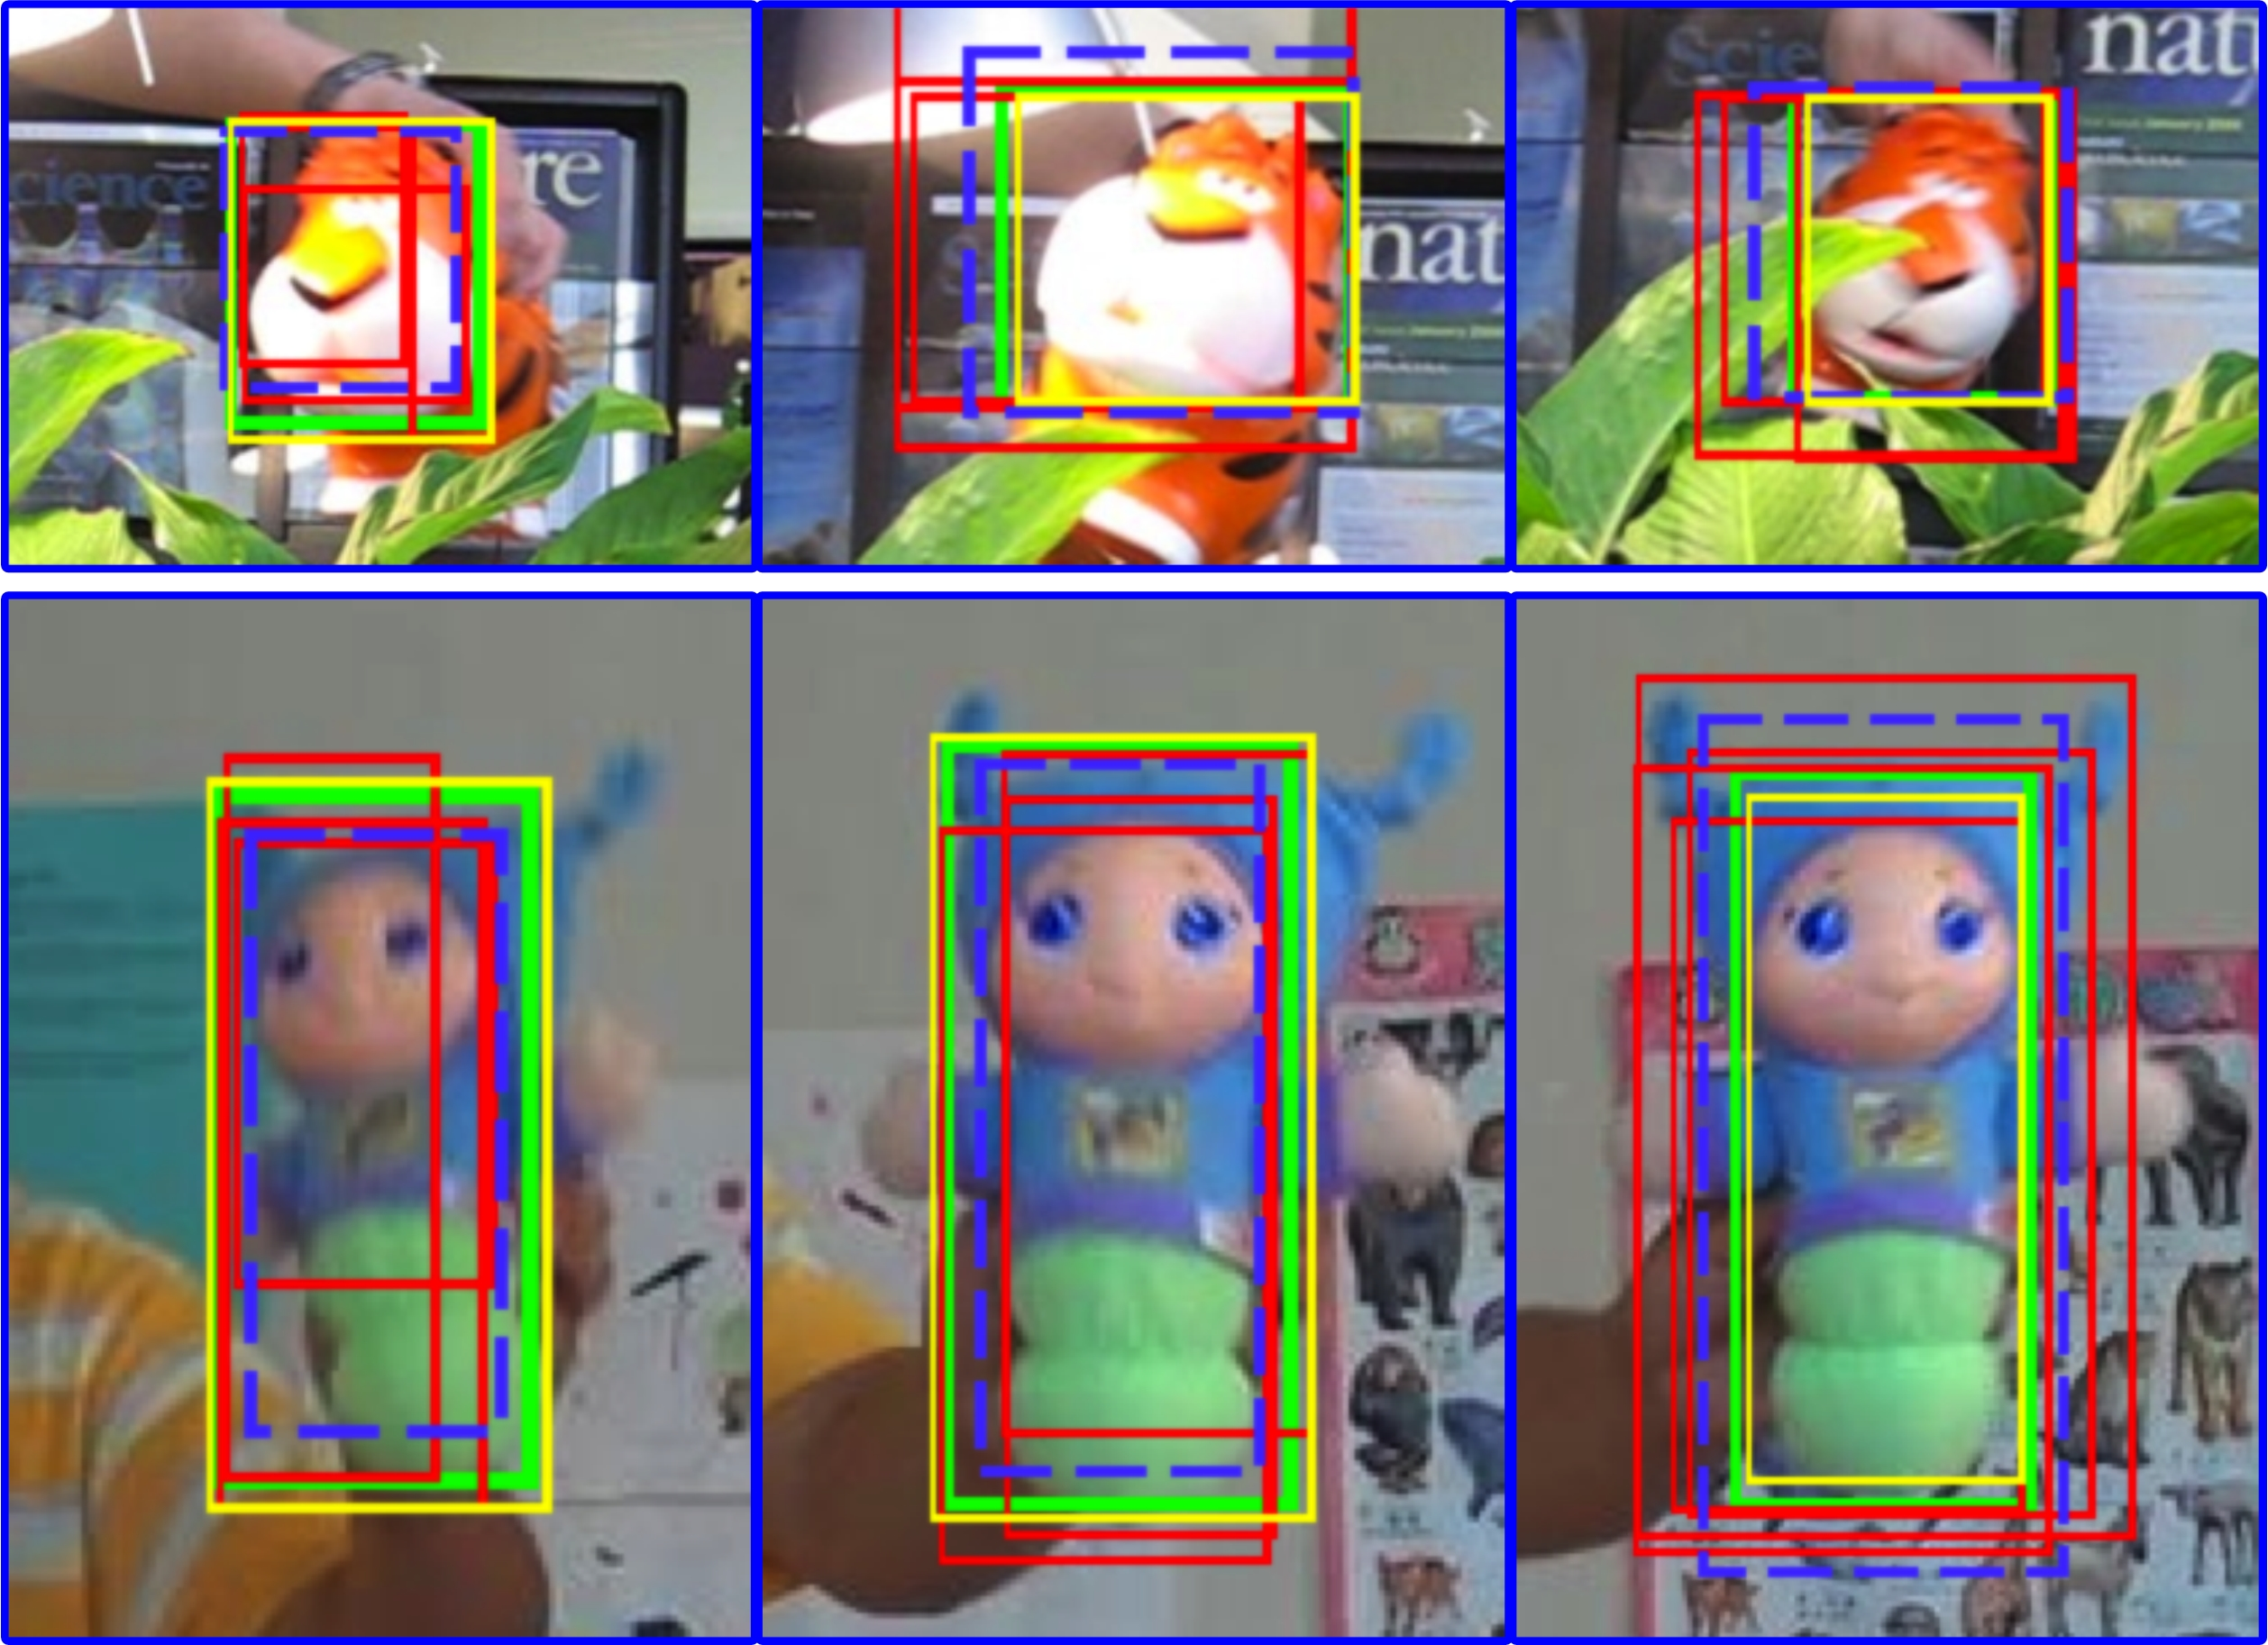
\includegraphics[width=10cm]{rejection.jpg}
	%	\vspace{-0.2in}
	\caption{目标候选辨别和带阻尼更新的可视化例子(图例见图\ref{process})}
	\label{rejection}
\end{figure}

\section{参数设置}
\label{param_setup}
从上文中可以看出,本章的跟踪算法引入了大量的参数。
这些参数对跟踪器的性能有着极大的影响,因此参数设置也是跟踪算法设计中至关重要的步骤。
简单粗暴地进行大范围的参数遍历,寻找能够在测试集上取得最优效果的参数组合,看似合理,但却是不可行的。
如果参数数目较多,各参数取值范围较大,若再加上测试集较大,那么参数遍历的时间开销将不可接受。
更重要的一点是,针对特定测试集遍历得出的参数设置很可能是过拟合的,难以适用于其它测试集或者实际场景。
因此,本节将尽量保留原版本KCF跟踪器和目标候选生成器EdgeBoxes的参数设置。
对于少数不适于本章算法的参数设置,则根据其实际意义进行微调。


在本章跟踪器的原KCF部分,除了两个参数以外,其它参数设置保持与原版KCF一致,例如尺度因子$s^d=2.5$(\ref{wholeprocesssec}节)、
高斯核函数带宽$\sigma=0.5$(公式\ref{kcf-kr})、规则化参数$\lambda=0.0001$(公式\ref{kcf_learning}、\ref{kcfdp-updating})。
需要调整的两个参数分别为回归目标矩阵$\mathbf{y}$的标准方差(公式\ref{kcf_learning}、\ref{kcfdp-updating})和学习速率$\eta$(公式\ref{kcfdp-updating}和公式\ref{kcf_appearlearning})。
如图\ref{regresstarget}所示,由于回归目标矩阵符合二维高斯函数,因此它的标准方差设置地越小,
$\mathbf{y}$的峰值部分就越陡峭,相关滤波器的辨别规则就会越严格。
如果相关滤波所使用的图像特征较为简单,那么标准方差就不宜设置地太小。
原因在于简单特征的不变性(如旋转不变性、尺度不变性等)普遍较差,
若辨别标准过于严格,在目标物体外观发生较大变化时就很可能无法发现目标,导致跟踪失败。
然而本章通过使用图像特征整合,获得了不变性较强的混合特征。
因此可以将标准方差适当减小,从``$0.1\times$图像对角线长度的平方根'',减小为``$0.06\times$图像对角线长度的平方根''。
通过减小标准方差,在成功检测到目标的情况下,获得的目标物体边界框将更加准确。
同样由于整合后的混合特征具有更强的不变性,学习速率$\eta$也从$0.02$下调到$0.01$,
使得跟踪器既能不断适应变化的目标外观,又不易受到目标遮挡和偶发跟踪误差的影响。

\begin{figure}[htb]
  \centering
  \subfloat[标准方差设置为$0.1\times$图像对角线长度的平方根]{%
    \label{regresstarget1}
    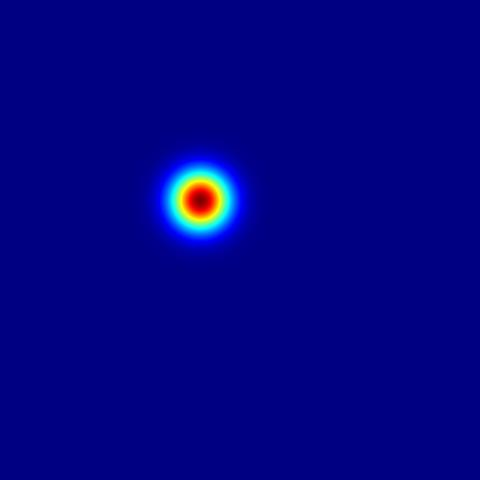
\includegraphics[height=4cm]{heatAfter}}\hspace{1cm}
  \subfloat[标准方差设置为$0.2\times$图像对角线长度的平方根]{
    \label{regresstarget2}
    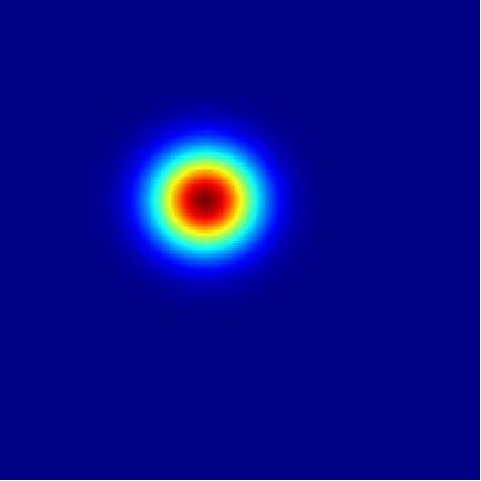
\includegraphics[height=4.05cm]{heatAfter2}}\hspace{0.2cm}
      \subfloat{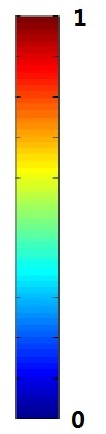
\includegraphics[height=4cm]{heatAfter3}}
  \caption{使用不同标准方差的相关滤波器回归目标矩阵}
  \label{regresstarget}
\end{figure}

在目标候选生成器部分,新参数$s^e$,即``尺度和宽高比检测窗口''的尺度因子,被设置为$1.4$。
此处$1.4$为$\sqrt{2}$的近似,它限制EdgeBoxes在一个两倍于目标图像块面积的窗口内寻找目标物体。
该参数设置即是假设:两帧间目标物体外表的面积最多扩大一倍。

至于EdgeBoxes本身,本节仅作简要介绍以便于分析参数设置,更详细的分析和优化将在下一章进行。
对于输入的图像,EdgeBoxes首先利用``结构化边界(Structured Edge)提取器\upcite{structurededge}''进行边界提取,
并计算出每个像素的边界响应值(属于物体边界的置信度)。
然后它以``滑动窗口''的形式遍历整幅输入图像,并对每一个窗口进行评分。
控制滑动窗口的参数有$stepSize$、$maxAspectRatio$和$minBoxArea$等。
$stepSize$是滑动窗口时,两个相邻窗口的IoU,用于控制采样密度。
所有窗口的宽高比均被限制在$1/maxAspectRatio$到$maxAspectRatio$之间,
而最小窗口的面积被限制为$minBoxArea$,因此这两个参数被用于控制目标候选可能的形状和大小。
对于每一个窗口,EdgeBoxes的评分函数为:
\begin{equation}
	h_b = \frac{\sum_{i\in b}w_{i}m_i}{2(b_w+b_h)^\kappa} - \frac{\sum_{p\in b^{in}}m_p}{2(b_w+b_h)^\kappa}. \label{edgeboxes}
\end{equation}
式中,$i$代表一个像素,其边界响应值记为$m_i$。
$b$即是待评分的窗口对应的图像块,其宽度和高度分别为$b_w$和$b_h$。
$b^{in}$是$b$的中心部分,大小为 ${b_w}/{2}\times {b_h}/{2}$。
$w_{i}\in [0,1]$是一个权值,代表着$i$所在的物体边界完全包含在$b$中的可能性。
显然$b$的尺度越大,其中包含的物体边界就越多,因此$\kappa$用于惩罚较大的窗口。
完成所有窗口的评分后,EdgeBoxes将对得分高于$minScore$的窗口进行进一步的细化和过滤,然后作为目标候选输出。

设置EdgeBoxes自身的参数时,本节基本保留其默认设置(以0.7为期望IoU),如$stepSize=0.65$。
但是,参数$minBoxArea$和$maxAspectRatio$将根据上一帧中目标物体边界框的大小,不断更新:
\begin{equation}
\begin{aligned}
	&minBoxArea=0.3\times w_{i-1}\times h_{i-1};\\
	&maxAspectRatio=1.5\times \max\{\frac{w_{i-1}}{h_{i-1}},\frac{h_{i-1}}{w_{i-1}}\}.
	\label{EBfactor}
\end{aligned}
\end{equation}
通过用上式控制滑动窗口的大小和形状,EdgeBoxes生成目标候选的速度将大大加快,并且避免了大量无用目标候选的产生。
此外,公式\ref{edgeboxes}中的$\kappa$从$1.5$轻微下调至$1.4$。
原因在于,物体检测任务中的物体可能位于任意位置、具有任意大小;但是在跟踪任务中,仅需要找出目标物体,
且目标物体通常占据了输入图像块的大部分面积。
因此$\kappa$需要适度减小,以减轻对于较大目标候选的惩罚。
本节对得分阈值$minScore$的修改较大,从$0.01$减小到了$0.0005$。
这是一种较为保守的参数设置,目的在于确保跟踪目标所在的目标候选不被滤除。
通过实际验证,EdgeBoxes在每一帧中平均生成约100个目标候选(最多时生成了277个)。
因此进入目标候选过滤的最大边界框数量,即算法\ref{algorithm}第5行的$N$,设置为200。
该参数设置既能保证获取到绝大部分目标候选,还能将它们用定长矩阵进行存储,提高计算效率。
最后,作为一个经验参数,公式\ref{kcfdp-damping}中的阻尼因子$\gamma$设置为0.7。

\section{实验结果与分析}
\subsection{实验设置}
为了表述方便,这里将本章提出的,融合了相关滤波器和目标候选生成器的新跟踪器命名为``KCFDP''(``Kernelized Correlation Filter with Detection Proposals'',即``加入了目标候选的核化相关滤波器'')。
实验将在著名的OTB(Object Tracking Benchmark)\upcite{50seqs, otbweb}测试集以及它的两个子集上进行,
结果评价标准采用通用的精确度图和成功率图,
用于对比的跟踪器共计达到了34个。
开放的大型测试集、通用的评价标准、以及庞大的对照组将共同保证本章实验的充分性和完备性。

\subsubsection{测试集和对照组构成}
本章的测试集来自著名的OTB,它包括了50个极具挑战性的视频序列(共计51个跟踪目标),其概览如图\ref{otb50}所示。
OTB还为每一个视频序列注明了其主要包含的跟踪障碍,例如``快速运动''、``遮挡''、``尺度变化''、``光照变化''等共计11种,
且一个视频序列可能包含多种跟踪障碍。
因此,将具有相同跟踪障碍的序列组成OTB的一个子集,即可用于测试跟踪器对该障碍的适应力和鲁棒性。
OTB提供的跟踪障碍中已有``尺度变化'',且共计有28个序列包含该障碍,因此这28个序列组成的子集将被用于评测KCFDP对于尺度的适应力。

\begin{figure}[htb]
	\centering
		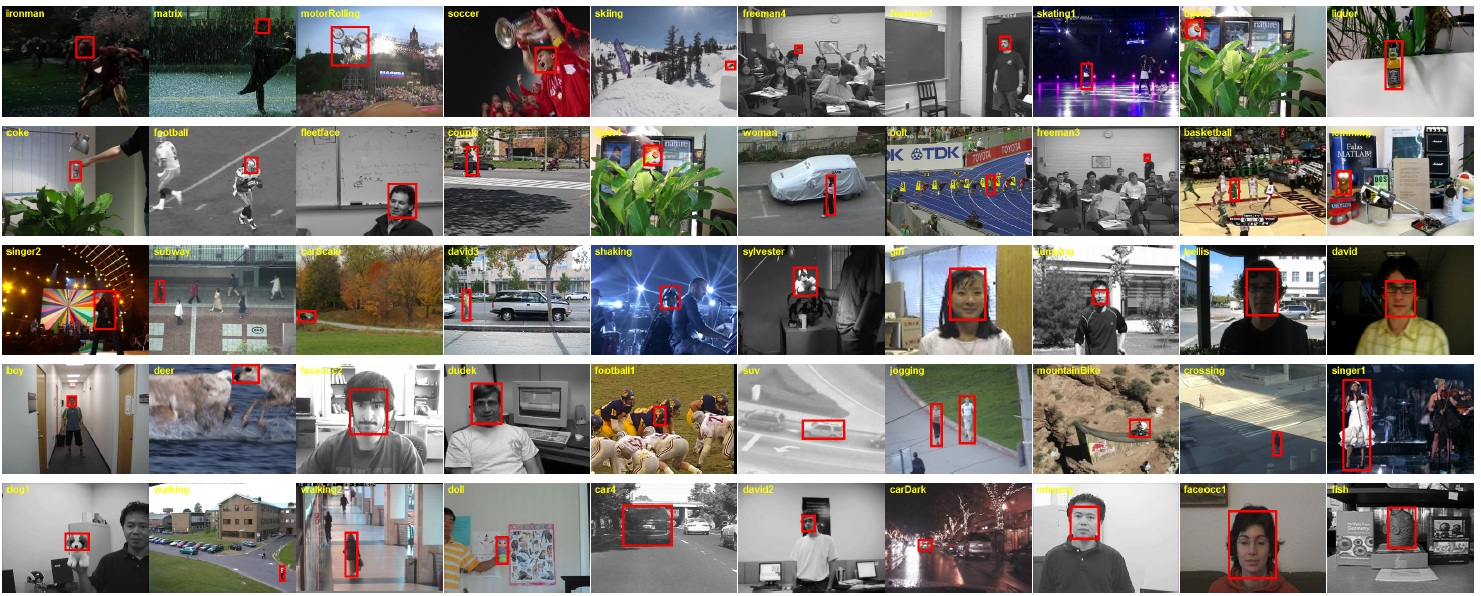
\includegraphics[width=14.5cm]{otb50.jpg}
	\caption{本章所使用的OTB\upcite{50seqs}测试集}
	\label{otb50}
\end{figure}

但是,OTB并没有标注``宽高比变化''这一障碍,因此本节将根据OTB给出的正确跟踪结果(Ground Truth),
即每一帧中紧密包围目标物体的边界框真值,自行进行提取。
判断一个视频序列包含``宽高比变化''障碍的标准如下。
如图\ref{aspseqs}所示,对于该视频的每一帧,将该帧的目标物体边界框和它的前30帧的目标物体边界框一一进行宽高比对比。
如果某次对比中,宽高比的比值超过了$[1/\sqrt{2}, \sqrt{2} ]$这一区间,则认为当前帧``正在经历宽高比变化''。
如果该视频序列有10\%以上的帧``正在经历宽高比变化'',则认为该序列中包含```宽高比变化''这一跟踪障碍。
根据该标准,一共有14个序列包含``宽高比变化''障碍,它们是:
\textit{Soccer}、\textit{Matrix}、\textit{Ironman}、\textit{Skating1}、\textit{Shaking}、\textit{Couple}、\textit{Girl}、
\textit{Walking2}、 \textit{Walking}、\textit{Freeman3}、\textit{Freeman4}、\textit{Skiing}、\textit{MotorRolling}和\textit{Woman}。
这些序列共有4560帧,其中1017帧``正在经历宽高比变化''。
它们组成的子集将被用于评测KCFDP对于宽高比变化的适应力。

\begin{figure}[htb]
	\centering
		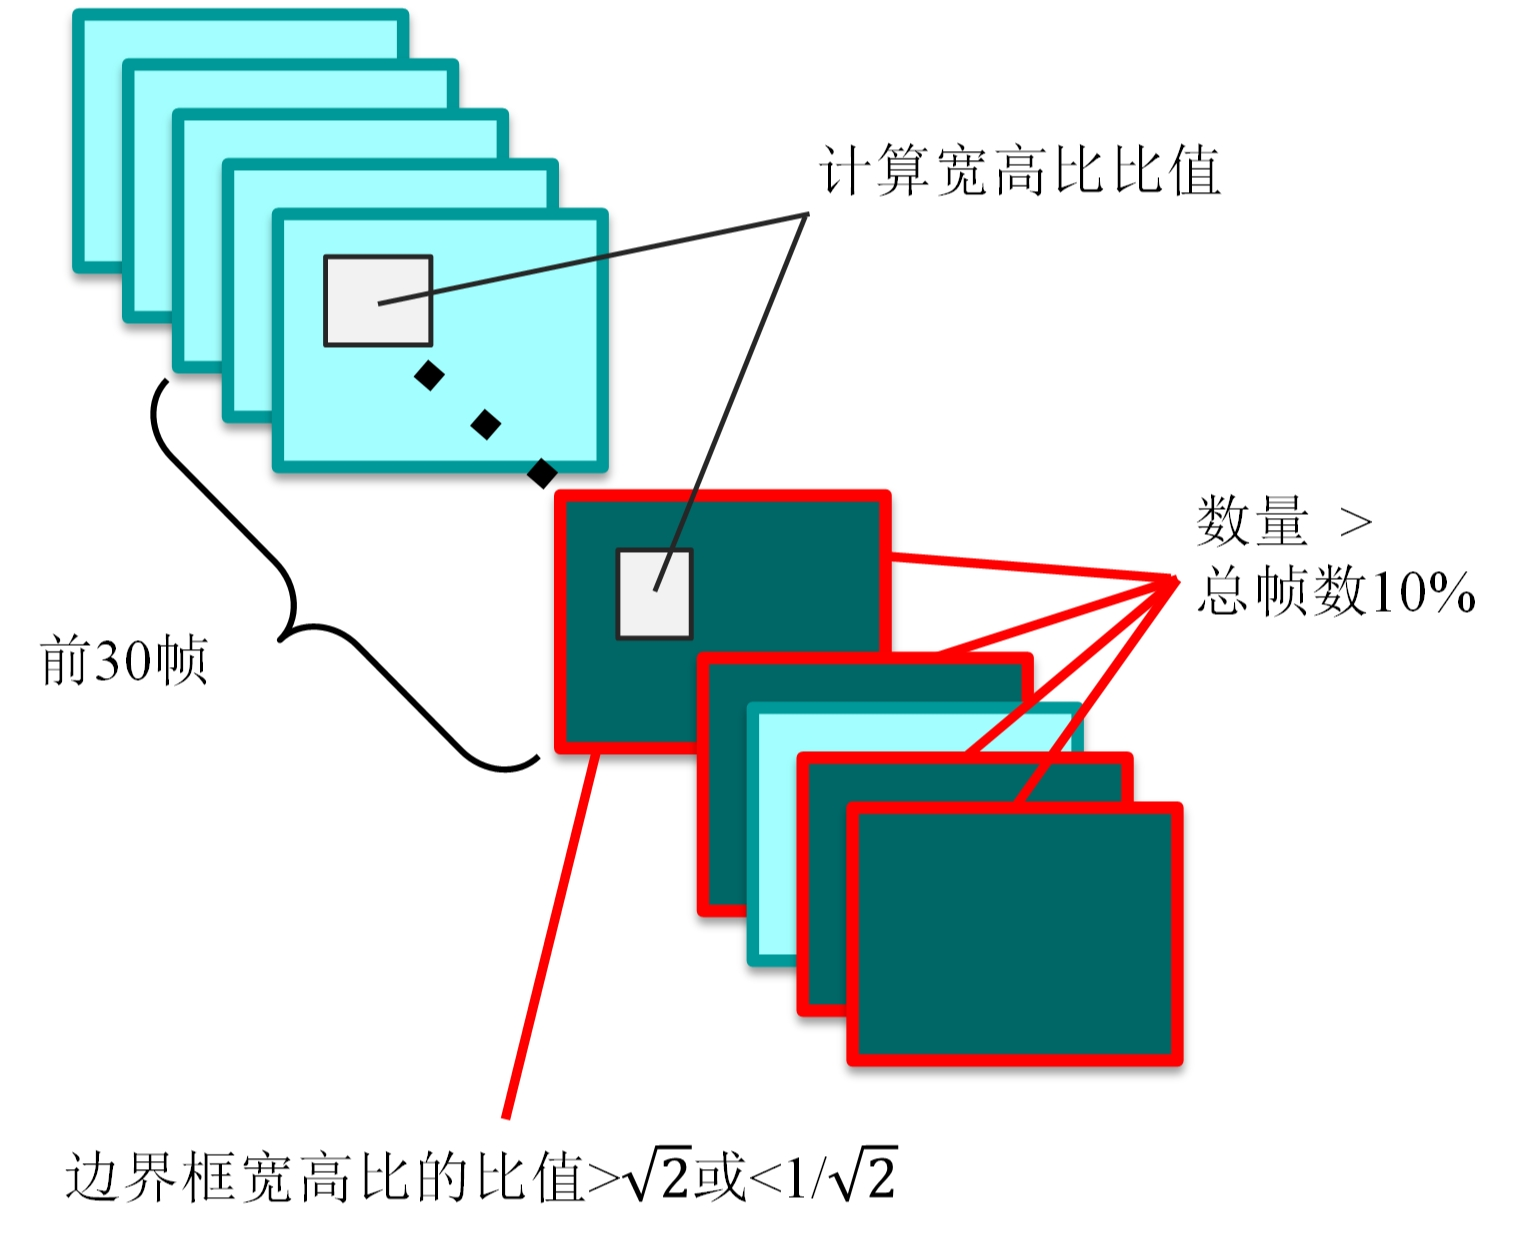
\includegraphics[width=8cm]{aspseqs.jpg}
	\caption{判断视频序列包含``宽高比变化''的过程}
	\label{aspseqs}
\end{figure}

OTB测试集除了提供了50个视频序列和正确的跟踪结果,还额外提供了29个跟踪器在它之上的运行结果。
这29个跟踪器中不乏
SCM\upcite{scm}、Struck\upcite{struck}、TLD\upcite{tld}、VTD\upcite{vtd}和ALSA\upcite{asla}等当前最为先进的跟踪器。
本节将直接利用这些跟踪器的运行结果,与KCFDP的结果进行对比评测。
此外,还有5个基于相关滤波的跟踪器被包含在对照组中,
即KCF\upcite{kcf}、DSST\upcite{dsst}、ACT\upcite{act}、SAMF\upcite{samf}和CKCF。
其中CKCF就是去除了目标候选生成器的KCFDP,也即是加入了图像特征整合和鲁邦更新的KCF。
综上,对照组中将共有34个跟踪器。

\subsubsection{评价标准}
在一些早期的工作中,通常使用平均中心位置误差(Averaged CLE)或者平均重叠率(Averaged IoU)来评价跟踪器的准确性。
平均中心位置误差即是在视频序列的所有帧中,计算跟踪器结果和正确跟踪结果中心间的距离,并进行平均。
显然,中心位置误差无法反映出尺度和宽高比是否准确。
平均重叠率进了一步,它用跟踪器结果和正确跟踪结果的IoU来替代中心位置误差。
但是,这两者最大的问题在于,当跟踪器丢失目标时,会对跟踪结果进行随机的惩罚,从而都无法准确反映跟踪器的准确性。

因此,本节将沿用\cite{50seqs}中提出的准确性评价标准,即使用准确率图(Precision Plot)和成功率图(Success Plot)。
要得到准确率图,需要先计算距离精度(Distance Precision)。距离精度的定义为:视频序列中中心位置误差小于某个阈值的帧所占的比例。
而成功率图则依赖于重叠精度(Overlap Precision),其定义为:视频序列中IoU大于某个阈值的帧所占的比例。
准确率图展示的是,在不同的中心位置误差阈值下(沿横坐标),跟踪器在所有序列上的平均距离精度(沿纵坐标)。
类似的,成功率图展示的是在不同的IoU阈值下(沿横坐标),跟踪器在所有序列上的平均重叠精度(沿纵坐标)。
对于准确率图,跟踪器将按照以20像素为阈值时的距离精度进行排名。
而对于成功率图,跟踪器将按照``曲线下方面积''(Area Under Curve,AUC)进行排名。

\subsection{尺度和宽高比适应力评测}
Resultant Precision Plots and Success Plots are shown in Fig.\ref{result-scale&aspect}, which shows our tracker is superior in both
scale and aspect ratio adaptability comparing to other trackers.
% More obvious superiority can be observed in Success Plots, which
%implies that the integration of detection proposals contributes mainly to the overlap rate between detected boxes and ground truths.


\subsection{整体性能评测}

\section{小结}
